%% IEEE conference draft. Compile from experiments/paper/ with:
%%   pdflatex main && bibtex main && pdflatex main && pdflatex main
%% Every number in Section III comes from data/ or from fit_results.json,
%% generated by experiments/run_experiments.py. Do not type numbers into the
%% body: \input the generated tables instead.

\documentclass[conference]{IEEEtran}

\usepackage{amsmath,amssymb}
\usepackage{amsthm}
\usepackage{booktabs}
\usepackage{array}
\usepackage{pgfplots}
\usepackage{siunitx}
\usepackage{tikz}
\usepackage{hyperref}
\usepackage{xcolor}

% The author's name is given in both scripts. pdfLaTeX has no CJK glyphs of its
% own, so the Chinese characters are set through CJKutf8's gbsn family; without
% this the name would be dropped at compile time as an unset Unicode character,
% which is a silent failure of exactly the kind the rest of the paper refuses.
\usepackage{CJKutf8}

\usetikzlibrary{arrows.meta,positioning}
\theoremstyle{definition}
\newtheorem{definition}{Definition}
\pgfplotsset{compat=1.17, table/col sep=comma}
\sisetup{detect-all}

% The topology figure's numbers. Generated, never typed: a drawing whose labels
% are hand-written is a drawing that lies the first time a fidelity changes.
% generated by experiments/run_experiments.py -- do not edit
\newcommand{\fidQuantum}{0.98}
\newcommand{\resQuantum}{0.02}
\newcommand{\ninesQuantum}{1.699}
\newcommand{\needsQuantum}{2}
\newcommand{\seamQuantum}{no}
\newcommand{\fidPhysicochemical}{0.95}
\newcommand{\resPhysicochemical}{0.05}
\newcommand{\ninesPhysicochemical}{1.301}
\newcommand{\needsPhysicochemical}{2}
\newcommand{\seamPhysicochemical}{no}
\newcommand{\fidBiological}{0.9}
\newcommand{\resBiological}{0.1}
\newcommand{\ninesBiological}{1.000}
\newcommand{\needsBiological}{2}
\newcommand{\seamBiological}{no}
\newcommand{\fidCognitive}{0.7}
\newcommand{\resCognitive}{0.3}
\newcommand{\ninesCognitive}{0.523}
\newcommand{\needsCognitive}{2}
\newcommand{\seamCognitive}{no}
\newcommand{\pathTrans}{0.5865}
\newcommand{\pathRes}{0.4135}
\newcommand{\depthPenalty}{0.600}
\newcommand{\perBoundaryBudget}{0.00251}
\newcommand{\epsPolicy}{1e-2}
\newcommand{\phaseFid}{1e-5}
\newcommand{\fnContrast}{98000}
\newcommand{\shortWorst}{Quantum$\mid$Physico-chemical}
\newcommand{\shortWorstNines}{0.30}


% The emergence section's numbers, from experiments/emergence_experiment.py.
% generated by experiments/emergence_experiment.py -- do not edit
\newcommand{\emK}{2.0400}
\newcommand{\emKstderr}{4.2e-16}
\newcommand{\emAlpha}{8.6202}
\newcommand{\emAlphastderr}{0.146}
\newcommand{\emAzero}{0.4091}
\newcommand{\emRtwoU}{1.000000000}
\newcommand{\emRtwoD}{0.8968}
\newcommand{\emSelectivity}{0.457}
\newcommand{\emKoverPzero}{0.78288}
\newcommand{\emWidth}{3.94}
\newcommand{\emSlope}{0.271}
\newcommand{\emPointsperdecade}{3.9}
\newcommand{\emFidTwenty}{0.880}
\newcommand{\emResTwenty}{0.120}
\newcommand{\emNinesTwenty}{0.92}
\newcommand{\emPtwoParams}{3.54e13}
\newcommand{\emPtweFactor}{1771}
\newcommand{\emPoneParams}{3.53e10}
\newcommand{\emPoneFactor}{1.8}
\newcommand{\emNearestDepth}{5}
\newcommand{\emNearestScale}{15.8}
\newcommand{\emCollapseError}{8e-16}
\newcommand{\emExponentRatio}{4.5}


% The causal section's numbers, from experiments/causal_experiment.py.
% generated by experiments/causal_experiment.py -- do not edit
\newcommand{\cgTasks}{1000}
\newcommand{\cgFailures}{302}
\newcommand{\cgAbsent}{197}
\newcommand{\cgStale}{105}
\newcommand{\cgPolluted}{525}
\newcommand{\cgFalseCompletionPct}{30}
\newcommand{\cgPollutionPct}{50}
\newcommand{\cgContextFcr}{100.0}
\newcommand{\cgContextFcrLow}{98.7}
\newcommand{\cgContextSens}{0.0}
\newcommand{\cgWeakFcr}{79.8}
\newcommand{\cgWeakSens}{20.2}
\newcommand{\cgWeakFar}{3.2}
\newcommand{\cgWeakCeiling}{20.7}
\newcommand{\cgWeakLeak}{0.41}
\newcommand{\cgCausalFcr}{0.0}
\newcommand{\cgCausalFcrHigh}{1.3}
\newcommand{\cgCausalSens}{100.0}
\newcommand{\cgDelta}{0.698}
\newcommand{\cgCausalBefore}{69.8}
\newcommand{\cgCausalAfter}{0.0}
\newcommand{\cgWeakBefore}{91.7}
\newcommand{\cgContextBefore}{100.0}
\newcommand{\cgContextGivenReject}{100}
\newcommand{\cgCausalGivenReject}{0}
\newcommand{\cgWeakGivenReject}{79.8}
\newcommand{\cgMissing}{197}
\newcommand{\cgMismatch}{105}
\newcommand{\cgIssued}{698}


% The falsification section's numbers, from
% experiments/true_emergence_experiment.py.
% generated by experiments/true_emergence_experiment.py -- do not edit
\newcommand{\teDepthMax}{6}
\newcommand{\teGridPoints}{49}
\newcommand{\teContamPct}{50}
\newcommand{\teAnchor}{$10^{5}$}
\newcommand{\teNinesNinetyNine}{2.02}
\newcommand{\teANinetyNine}{$1655$}
\newcommand{\teAFcrNinetyNine}{100}
\newcommand{\teAFcrDepthOne}{98.1}
\newcommand{\teBCrossNinetyNine}{$7.94\times10^{-8}$}
\newcommand{\teBRateNinetyNine}{$7.94\times10^{-13}$}
\newcommand{\teNestedCrossNinetyNine}{$160$}
\newcommand{\teBNestedRate}{$1.60\times10^{-3}$}
\newcommand{\teBOrders}{9.3}
\newcommand{\teInflationDeep}{$2.08\times10^{10}$}
\newcommand{\teGapDepthOne}{$52.5$}
\newcommand{\teAFloor}{$1572$}
\newcommand{\teAFloorLimit}{$1562$}
\newcommand{\teBFloor}{$1.00\times10^{-13}$}
\newcommand{\teCollapseNines}{0.85}
\newcommand{\teCollapseD}{0.858}
\newcommand{\teSlopeA}{0.41}
\newcommand{\teSlopeB}{6.00}
\newcommand{\teSlopeBNested}{1.00}


% The solidification section's numbers, from
% experiments/solidification_experiment.py.
% generated by experiments/solidification_experiment.py -- do not edit
\newcommand{\sdDepth}{10}
\newcommand{\sdRuns}{1000}
\newcommand{\sdVerifyCost}{1.00}
\newcommand{\sdCachedCost}{0.01}
\newcommand{\sdDetectCost}{0.02}
\newcommand{\sdGain}{100}
\newcommand{\sdColdUnlabelled}{10.00}
\newcommand{\sdColdLabelled}{1.27}
\newcommand{\sdColdPure}{1.09}
\newcommand{\sdColdPureRatio}{9.17}
\newcommand{\sdColdRatio}{7.87}
\newcommand{\sdWarmUnlabelled}{1.00}
\newcommand{\sdWarmLabelled}{0.03}
\newcommand{\sdRatio}{32.29}
\newcommand{\sdBound}{33}
\newcommand{\sdDepthGain}{33}
\newcommand{\sdSlopeUnlabelled}{32.39}
\newcommand{\sdSlopeUnlabelledRsq}{0.879}
\newcommand{\sdSlopeBudget}{3.3219}
\newcommand{\sdSlopeBudgetRsq}{1.000}
\newcommand{\sdSlopePredicted}{3.3219}
\newcommand{\sdNaiveFcr}{99}
\newcommand{\sdNaiveRho}{0.1}
\newcommand{\sdReplayRate}{90}
\newcommand{\sdCascadeRate}{35}
\newcommand{\sdBreakEvenRho}{0.97}
\newcommand{\sdRhoCascadeTen}{0.176}
\newcommand{\sdRhoCascadeHundred}{0.019}
\newcommand{\sdCascadePenalty}{4.46}
\newcommand{\sdCompiledRungs}{10}
\newcommand{\sdCrossedRungs}{10}
\newcommand{\sdBreakEven}{0.99}


% The critical-budget section's numbers, from
% experiments/critical_budget_experiment.py.
% generated by experiments/critical_budget_experiment.py -- do not edit
\newcommand{\cbBar}{0.1090}
\newcommand{\cbGain}{9.174}
\newcommand{\cbGainTwo}{1.803}
\newcommand{\cbCritBudgetZero}{1.000}
\newcommand{\cbCritBudgetDetector}{1.0230}
\newcommand{\cbCritBudgetRhoZero}{1.0206}
\newcommand{\cbCritBudgetRhoHalf}{1.0421}
\newcommand{\cbCritBudgetRhoNine}{1.2532}
\newcommand{\cbSlopeInfra}{1.1246}
\newcommand{\cbSlopePredicted}{1.1223}
\newcommand{\cbIntercept}{1.0000}
\newcommand{\cbSlopeRsq}{1.000000}
\newcommand{\cbCritBudgetGranular}{2.020}
\newcommand{\cbDetectorLimit}{0.891}
\newcommand{\cbDriftLimit}{0.980}
\newcommand{\cbPremiumLimit}{8.47}
\newcommand{\cbCbarDetector}{0.1290}
\newcommand{\cbCritBudgetCdHalf}{2.279}
\newcommand{\cbCritBudgetCdHigh}{21.73}
\newcommand{\cbPeakBudget}{3.71}
\newcommand{\cbPeakRatio}{2.4}
\newcommand{\cbPeakPower}{7}
\newcommand{\cbPeakLog}{7.38}
\newcommand{\cbDepthSlope}{8.174}
\newcommand{\cbKnot}{10}
\newcommand{\cbHorizonExp}{12}
\newcommand{\cbAlpha}{27.63}
\newcommand{\cbLocalRate}{20.437}
\newcommand{\cbSlopeAtTen}{25806.9}
\newcommand{\cbSlopeAtSixty}{1.071}
\newcommand{\cbSlopeAtHundred}{1.0002}


% The nested-solidification section's numbers, from
% experiments/nested_solidification_experiment.py.
% generated by experiments/nested_solidification_experiment.py -- do not edit
\newcommand{\nestedLookup}{0.109}
\newcommand{\nestedGain}{9.174}
\newcommand{\nestedBranch}{4}
\newcommand{\nestedKnee}{0.75}
\newcommand{\nestedPremium}{5}
\newcommand{\nestedBstar}{6.61}
\newcommand{\nestedBstarGranular}{6.08}
\newcommand{\nestedBuild}{39.23}
\newcommand{\nestedBrec}{39.23}
\newcommand{\nestedFlatCost}{4096}
\newcommand{\nestedMarginalNested}{0.109}
\newcommand{\nestedMultipleMantissa}{3.76}
\newcommand{\nestedMultiplePower}{4}
\newcommand{\nestedEffFar}{30207}
\newcommand{\nestedBaseHalf}{2.0}
\newcommand{\nestedBaseNinety}{4.00}
\newcommand{\nestedMultipleDeep}{6.01}
\newcommand{\nestedMultipleDeepExp}{5}


% The self-audit appendix's numbers, from experiments/paper_self_audit.py.
% generated by experiments/paper_self_audit.py -- do not edit
\newcommand{\saPassCount}{7}
\newcommand{\saInvalidCount}{2}
\newcommand{\saUnavailableCount}{2}
\newcommand{\saBlindCount}{1}
\newcommand{\saFailCount}{0}
\newcommand{\saClaimCount}{12}
\newcommand{\saStrataCount}{5}
\newcommand{\saEdgeCount}{4}
\newcommand{\saPairCount}{10}
\newcommand{\saUnwitnessedCount}{6}


% The bibliography audit's numbers, from experiments/citation_audit_report.py.
% generated by experiments/citation_audit_report.py -- do not edit
\newcommand{\caTotal}{19}
\newcommand{\caPass}{17}
\newcommand{\caFail}{0}
\newcommand{\caInvalid}{2}
\newcommand{\caCrossrefCount}{13}
\newcommand{\caArxivCount}{4}
\newcommand{\caAgencyCount}{2}
\newcommand{\caPriorPass}{0}
\newcommand{\caPriorInvalid}{19}
\newcommand{\caLocatedCount}{2}


\hypersetup{colorlinks=true,linkcolor=black,citecolor=black,urlcolor=blue,
  pdftitle={Fractal Interfaces: A Quantitative Model of Cross-Scale Boundaries},
  pdfauthor={Zhizhi Liao},
  pdfsubject={Cross-scale interfaces, difficulty, reach, and the economics of
    solidification},
  pdfkeywords={interfaces, cross-scale, power law, quantum biology,
    critical budget, nested reuse}}


% Two-column pages carrying a full-width float cannot be justified to the last
% line: the float fixes the column height and the remaining text is broken to fit
% it, leaving glue to stretch. Ragged bottoms are the honest rendering of that,
% and they remove the underfull-box warnings without moving a single word.
\raggedbottom

\begin{document}

\title{Fractal Interfaces: A Quantitative Model of Cross-Scale Boundaries,\\
Calibrated on Biological Quantum Coherence}

\author{\IEEEauthorblockN{Zhizhi Liao (\begin{CJK}{UTF8}{gbsn}廖至智\end{CJK})}
\IEEEauthorblockA{Independent Researcher\\
liaozhizhi@foxmail.com}}

\maketitle

\begin{abstract}
Interfaces are usually described as application programming interfaces: generic,
symmetric, and cheap to cross. Between physical layers this description fails. We
formalise an interface as a \emph{gap}---a narrowing condition whose satisfaction
buys reach---and derive the consequences instead of asserting them. A
twelve-decade coherence gap between a warm biological layer and a quantum layer is
mapped to a difficulty $D=1-e^{-P/P_0}$ with $P_0$ fixed by that single real gap,
and reach amplification is modelled as inverse rarity, $A=s^{-n}$, where $s$ is the
fidelity of the narrow condition and $n$ the number of independent constraints.
The model then predicts a power law $\mathrm{Reach}\propto(1-D)^{-k}$ with
$k=\gamma P_0\lvert\ln s\rvert$. We run \num{7000} simulated crossings across three
experiments, and two further experiments that price the boundary itself. The
results are quantitative, and two of them are negative. (i)~A cryostat that extends
coherence by $10^{9}$ gains $10^{2}$ in reach; a protein that extends it by
$10^{0}$ gains $10^{5}$---reach tracks replicability, not coherence time.
(ii)~No single $\mathrm{Reach}=f(D)$ exists: the best two-parameter single curve
explains \num{33}\% of the variance where no history is present and \num{12}\%
once history is included, whereas the conditional law recovers its exponent to
within \num{1.1}\% with $R^2\approx0.998$. (iii)~The failure boundary is the
mechanism's fidelity, not a universal difficulty: $D=0.999$ is a crash point only
for a \num{99.9}\%-faithful mechanism. (iv)~Fidelity is a property of a boundary
\emph{and a function}: the same quantum--chemical boundary routes excitations at
$0.98$ and preserves electronic phase at $10^{-5}$. Defining an interface as
seamless when its resistance $R=1-F$ falls below $\varepsilon$ makes seamlessness a
\emph{quantised} verdict---it flips at whole numbers of nines, not gradually---and
makes depth cost $\log_{10}n$ extra nines. Measured against a five-stratum stack,
no boundary is seamless, the quantum one is short by \num{0.30} nines, and the
adjacent stratum rather than the thermal bath is the binding noise source. Finally,
the widely reported exponential form of the law is shown to be exact in the
narrowing coordinate and along the ladder, local in difficulty with a rate
$k/(1-D)$ that diverges, and \emph{impossible} globally with a constant rate
because $\ln\mathrm{Reach}$ is strictly convex. The local rate converges as
$1+f^{2}/5$, which a least-squares fit confirms to five digits. A final experiment
maps a published language-model scaling law onto the same law, and finds the
mechanism usually offered for ``emergent'' capability to be wrong while the law
survives: the critical scale is real, but at it the per-boundary fidelity is
\num{\emFidTwenty}, not \num{0.99}, and the model's transition is four decades wide and
independent of task depth---so the reported step is what a smooth ramp looks like
when model sizes are sampled a decade apart. Running the
experiments then exposed three silent defects in the auditing engine itself,
including a witness digest that did not bind the gap's difficulty---two distinct
claims sharing one witness, which is the precise failure the model exists to
detect. All three are reported with reproductions. A last experiment asks whether
the alternative to a witness---a judge reading the agent's own report---can be
repaired. It cannot: on \num{\cgTasks} tasks the report-only judge passes every
failure, and the log-reading judge's ceiling is set by the logging fidelity of the
party under audit. Deleting the artefact while holding the context byte-identical
moves the causal judge from \num{\cgCausalBefore}\% to \num{\cgCausalAfter}\% and
the other two by exactly zero. A final experiment turns that witness on the paper's
own remedy: labelling turns depth into no explosion---completion of a ladder is
bounded by its prefixes---but removes a false prosperity of $10^{10}$ at
$D=0.99$. A closing experiment answers the question that refutation leaves open.
The falling marginal cost of depth is not a discount on probability but
\emph{solidification}: a rung crossed against a witness is compiled, so it pays for
the boundary that is new rather than for the prefix, and total cost grows as
$\log K$ rather than $K$---a fitted slope of \sdSlopeBudget{} against a predicted
$1/\log_{10}2=\sdSlopePredicted$ that nothing was fitted to. The exponential the
refutation forbids in cost per unit depth reappears, correctly placed, in reach per
unit budget; and seamlessness is the limit $\rho\to0$ of the compiled share, not a
property any drifting system holds. Turning that mechanism into a decision adds the
paper's only threshold with a closed form---and a negative result attached to it. A
compiled path that carries a fixed premium $S$ repays it only above
$B^{*}=c_v+S\,G_\infty/(G_\infty-1)$, a line whose intercept is the price of one
crossing and whose slope is fixed by the same price ratio; a monitor makes the
threshold rise with drift to a vertical asymptote at $\rho=1-c_d/(c_v-c_c)$. With
no premium the threshold collapses to $c_v$ itself, so the natural intuition---an
upfront verification makes compiling lose at small budgets---is false, and the
compiled system is never behind anywhere. Reach then tells the opposite story to
depth: the depth advantage grows without bound, while the reach advantage peaks at a
finite budget and returns to one at the horizon. We also prove that, unlike simple
amortisation---bounded at $G=\nestedGain$---the cross-layer reuse rate $\kappa$ is
the source of genuine exponential compound interest in interface evolution: the
marginal cost of a task spanning $d$ levels grows with base
$\min\!\bigl(L,1/(1-\kappa)\bigr)$, so compounding disappears below
$\kappa^{*}=1-1/L$ and saturates above it. We state explicitly what these
experiments do \emph{not} show.
\end{abstract}

\begin{IEEEkeywords}
cross-scale interfaces, quantum biology, fractal hierarchy, power laws, model
validation, negative results, compilation, critical budget, nested reuse
\end{IEEEkeywords}

\section{Introduction}

An interface is commonly treated as a contract: a published surface with two
sides, unchanged by what crosses it. That metaphor is useful for software and
misleading for everything else. Between a warm, wet, noisy biological layer and a
quantum layer, the boundary is not a surface but a \emph{narrowing}: almost nothing
fits through it, and what does fit through does not emerge unchanged on the other
side. Calling such a boundary an interface without saying what has to be true to
cross it is a category error dressed as a diagram.

Two habits keep the error alive. The first is explanatory circularity: an
interface is explained by its ``medium'', and the medium is then explained by
being the thing that carries the signal. Air is not the substrate of a
conversation; air is a layer, and a language fits through a very narrow opening in
it. Every medium is the next layer up, mistaken for a floor because that is where
the search stopped. The second habit is generic coupling: if two layers interact,
the interaction is assumed to be a matter of degree. Between physical layers the
interaction is usually a matter of \emph{existence}---the condition is either
satisfied or the crossing does not happen at all.

Hierarchy and self-similarity are old observations about complex systems
\cite{simon1962,mandelbrot1982}, and scaling laws recur across biology and across
networks \cite{west1997,barabasi1999}. This paper takes the second claim seriously
and makes it computable. We treat an
interface as a gap with a difficulty, a span (the set of sites where the two layers
can coexist at all), and a narrow condition whose satisfaction multiplies the
span. Crossing is not free and not symmetric: it buys reach at the cost of
satisfying something almost nothing satisfies.

\subsection{Relation to prior work}
\label{sec:related}

The claim that apparent capability jumps are an artefact of the metric is now
well established \cite{schaeffer2023,du2024,zhao2025}, and the emergence claim it
answers was stated explicitly \cite{wei2022}. Fractal structure has been used as
an analytic lens on language and on training dynamics
\cite{alabdulmohsin2025,torkamandi2025}, an agent's self-report is studied as a
control problem under subversion \cite{greenblatt2023,vanderweij2024}, and the
economics of when a claim is worth verifying at all already has a frontier of its
own \cite{gill2026}. None of these models the interface itself: none gives a
crossing a difficulty, a span and a narrowing condition, and none derives a reach
law from them. To our knowledge this is the first account in which the fractal
interface supplies the exponent and the causal label supplies the verdict, so that
``it works'' and ``it says it works'' are separated by construction rather than
by a better judge. Our $B^{*}$ is not the first verification threshold---%
\cite{gill2026} derives one on claim value---but it is a threshold on
\emph{depth}, and it moves only when the compiled regime pays a premium the
unlabelled one does not (\S\ref{sec:criticalbudget}); the compile-once,
check-cheaply economy that we later formalise as $\kappa$ is older than this paper
\cite{necula1997}, and we say so where we use it.

\subsection{Why biology is the test case}

Photosynthetic pigment--protein complexes are the best-documented candidate for a
system in which a macroscopic organism exploits a quantum layer. Two-dimensional
electronic spectroscopy reported long-lived oscillations in the Fenna--Matthews--Olson
(FMO) complex \cite{engel2007,brixner2005}, initially interpreted as electronic
coherence surviving at cryogenic temperatures
\cite{panitchayangkoon2010}. That interpretation was later challenged: the
long-lived beats do not survive to physiological temperature, and the residual
room-temperature oscillations are assigned to vibrational rather than electronic
coherence \cite{duan2017}. Meanwhile the excitation-trapping efficiency of FMO is
reported at \num{0.95}--\num{0.99} \cite{adolphs2006}, and noise-assisted transport
models show that dephasing can \emph{assist} rather than destroy transfer
\cite{mohseni2008,plenio2008,lambert2013,romero2017}.

This combination is exactly what a quantitative interface model needs, and it
points the opposite way from the popular story. The protein does not buy a longer
coherence time at room temperature---by the sceptical reading it buys none at all.
It buys \emph{reach}: the condition is instantiated wherever a cell is, rather
than wherever a dilution refrigerator is. A model that rewards reach in proportion
to coherence time gets the biology backwards, and we show numerically that it does.

\subsection{Contributions}

\begin{enumerate}
\item A formalisation of an interface as a gap, with difficulty, span, narrow
condition, and an explicit separation between whether a crossing \emph{held}
(verdict) and how far it \emph{carried} (status).
\item A derivation of the fractal amplification law
$\mathrm{Reach}\propto(1-D)^{-k}$, $k=\gamma P_0\lvert\ln s\rvert$, from an
inverse-rarity assumption, together with the statement that the exponent is
\emph{not} universal but indexed by fidelity.
\item Three computational experiments over \num{7000} crossings that test the law,
compare it against rival functional forms, and locate two distinct boundaries: a
statistical one at the mechanism's fidelity and a representational one at
$D=1-10^{-9}$.
\item A negative result, reported as such: there is no single
$\mathrm{Reach}=f(D)$, and the hypothesis that $D=0.999$ is a universal crash
point is false as stated.
\item A definition of \emph{seamlessness} as a threshold on boundary resistance
$R=1-F$, from which two things follow without further assumption: the verdict is
quantised in nines, and depth costs $\log_{10}n$ extra nines. Fidelity is shown to
be a property of a boundary \emph{and a function}, so that one boundary carries
two fidelities five orders apart.
\item A complete account of the exponential form of the law. It is exact in the
narrowing coordinate and along the ladder, local in difficulty with a rate
$k/(1-D)$ that diverges, and impossible globally with a constant rate, since
$\ln\mathrm{Reach}$ is strictly convex in $D$. The local rate's error is derived
($1+f^{2}/5$) and measured to five digits.
\item An application of the law to a published language-model scaling law, and a
refutation of the mechanism by which that law is usually said to explain
``emergence''. The critical scale is real but is not a fidelity threshold; it is
where a task of a given compositional depth crosses a given scoring bar. The
transition produced by the model is \emph{four decades wide and independent of
task depth}, so the apparent step is an artefact of sampling model sizes a decade
apart. This yields a falsifiable prediction about the width at two task depths.
\end{enumerate}

Section~\ref{sec:model} develops the model, including the definitions of fidelity
and of the seamless limit, Section~\ref{sec:exp} reports the experiments,
Section~\ref{sec:disc} discusses what the boundaries mean and what would falsify
the account, and Section~\ref{sec:concl} concludes.

\section{Mathematical Model}
\label{sec:model}

\subsection{Layers and gaps}

A \emph{layer} $L$ is a scale of description, carrying declared measurements
$\mu_L(q)$ for quantities $q$ in whatever unit $q$ names. A layer is not a medium:
it is a level, and all structure that matters lives on the gap between two of them.

An \emph{interface} between layers $A$ and $B$ is a tuple
$(c, S, D)$: a narrow condition $c$, an initial span $S$ (the number of sites where
$A$ and $B$ coexist without any crossing), and a difficulty $D\in[0,1)$. The span
is not a distance; it is a count of coexistence sites, so it can be multiplied.

\subsection{Potential and difficulty}

Let $P$ be the gap's \emph{potential}, the base-ten logarithm of the mismatch in
the quantity that matters, expressed in decades. For the macro/quantum coherence
gap, $P=12$ ($\SI{1}{\second}$ against \SI{1}{\pico\second}).

Difficulty saturates:
\begin{equation}
D(P) \;=\; 1-\exp\!\left(-\frac{P}{P_0}\right), \qquad
P(D) \;=\;-P_0\ln(1-D).
\label{eq:difficulty}
\end{equation}
Saturation rather than proportionality is forced by the requirement $D<1$: a gap
at difficulty exactly $1$ is a wall, and a wall is not an interface. Inverting
\eqref{eq:difficulty} requires $D<1$, a fact Section~\ref{sec:boundary} turns into
a measured boundary.

The scale $P_0$ is not a free parameter. Fixing the one real gap at the value the
model was specified with, $D(12)=0.99$, gives
\begin{equation}
P_0 \;=\; \frac{12}{-\ln(1-0.99)} \;=\; 2.6058\ \text{decades}.
\label{eq:p0}
\end{equation}
One observed gap, one calibration constant, no fitting.

\subsection{Narrow conditions, slack, and replicability}

A \emph{narrow condition} $c$ is a mechanism plus an artefact that a third party
could look up. Two of its properties do the work:

\begin{itemize}
\item \textbf{slack} $s\in(0,1)$: the fraction of the maximal coincidence actually
achieved. A protein that folds correctly \num{95}\% of the time has $s=0.95$.
\item \textbf{replicability} $r\in\{\text{true},\text{false}\}$: whether the
condition can be instantiated on the target layer \emph{at scale}. A cryostat is
a real crossing that cannot be repeated a billion times; a protein is a real
crossing that can.
\end{itemize}

The model refuses the combination $r=\text{false}$ with a large amplification: a
condition that cannot be instantiated at scale cannot buy scale. The contradiction
belongs to the claim, not to the auditor.

\subsection{Reach and the amplification law}

Suppose a crossing requires $n$ independent constraints, each satisfied at a
fraction $s$ of the target sites. Then a fraction $s^{n}$ of sites satisfy all of
them, and a crossing that works only there reaches $s^{-n}$ times further than one
that works anywhere. This is the model's central assumption: \emph{reach is
inverse rarity}. It is an assumption, not a thermodynamic result, and
Section~\ref{sec:threats} treats it as such.

With $n$ taken proportional to the gap's complexity,
\begin{equation}
n(P) \;=\; \max\!\left(1,\left\lceil \gamma P \right\rceil\right),
\qquad
A(s,n) \;=\; s^{-n},
\label{eq:amp}
\end{equation}
so the reach after crossing is
\begin{equation}
\mathrm{Reach} \;=\; \min\!\left(S\,A(s,n),\; H\right),
\label{eq:reach}
\end{equation}
where $H$ is a finite horizon beyond which further reach is not modelled.

Substituting \eqref{eq:difficulty} into \eqref{eq:amp} gives the
\emph{fractal amplification law}:
\begin{equation}
\ln A \;=\; \gamma P_0\,\lvert\ln s\rvert\,\bigl[-\ln(1-D)\bigr],
\quad\text{i.e.}\quad
A \;=\; (1-D)^{-k},
\label{eq:law}
\end{equation}
with
\begin{equation}
k \;=\; \gamma P_0\,\lvert\ln s\rvert .
\label{eq:k}
\end{equation}

A power law is an easy thing to over-claim: many reported exponents fail proper
distributional tests \cite{clauset2009}. We therefore make no discovery claim.
Equation~\eqref{eq:law} is \emph{derived} from \eqref{eq:amp}, and the regressions
in Section~\ref{sec:exp} test whether the implementation realises the derivation
and where it stops, not whether nature prefers a power law.

Two consequences follow before any data is collected, and both are falsifiable.
First, there is \emph{no} single $\mathrm{Reach}=f(D)$: the exponent depends on the
mechanism's fidelity, so the correct object is a one-parameter \emph{family} of
power laws indexed by $s$. A single curve fitted across mixed fidelity is the wrong
model, and Section~\ref{sec:law} shows it fits worse. Second, $k$ does not depend
on the generation: a law that is genuinely fractal must produce the same exponent
at every rung.

\subsection{Verdict and status}

Two questions are routinely conflated. \emph{Did the claim hold?} is a verdict:
PASS, FAIL, or INVALID (nothing was offered that could be refuted). \emph{How far
did it carry?} is a status: NARROW $(\le 10\times$, or not replicable) or
EXPANSIVE. A cryostat that closes a gap for one laboratory has verdict PASS and
status NARROW. Recording it with one word either slanders the refrigerator or
flatters it; both readings get the engineering wrong.

\subsection{Self-similarity}
\label{sec:selfsim}

Crossing closes the old gap and opens a new one of the same shape with a narrower
opening. The engine's nesting rule halves the remaining room,
\begin{equation}
D_{g+1} \;=\; D_g + \tfrac{1}{2}\left(1-D_g\right),
\label{eq:nest}
\end{equation}
so difficulty strictly rises, reach strictly grows, and the chain is self-similar
by construction. Equation~\eqref{eq:nest} is also where the representation
eventually fails; see Section~\ref{sec:boundary}.

\subsection{Fidelity, resistance, and why an interface disappears}
\label{sec:fidelity}

The model so far prices a crossing by its difficulty. It does not say what the
boundary \emph{costs}, and without that the phrase ``the interface became
transparent'' has no referent. We therefore attach to each boundary a fidelity
$F\in(0,1]$ and call $R=1-F$ its \emph{resistance}.

The first thing to establish is that $F$ is not a property of the boundary alone.
It is a property of the boundary \emph{and of what is being carried across it}. At
the quantum--chemical boundary of the photosynthetic apparatus two functions are
served by the same physical structure and they do not have the same fidelity. The
fraction of excitations that arrive at the reaction centre is
$F_{\text{route}}=0.98$, the FMO trapping efficiency \cite{engel2007}. The
fraction of electronic phase that survives the same crossing is
$F_{\text{phase}}\approx 10^{-5}$, because the electronic coherence time at
physiological temperature is $\SI{1}{\pico\second}$ \cite{duan2017} against the
$\SI{100}{\nano\second}$ an operating device would need. Two fidelities, five
orders of magnitude apart, one boundary. A model that reports a single $F$ per
boundary is not simplifying; it is answering a question nobody asked.

\begin{definition}[Seamless]
For a boundary $b$, a function $f$, and a policy threshold $\varepsilon\in(0,1)$,
the interface is \emph{seamless} for $(b,f)$ when
\begin{equation}
R_f(b) \;=\; 1-F_f(b) \;<\; \varepsilon .
\label{eq:seamless}
\end{equation}
\end{definition}

\paragraph{The verdict is quantised} A resistance of the form $R=10^{-p}$ has $p$
\emph{nines} of fidelity, and \eqref{eq:seamless} becomes $p>\log_{10}(1/\varepsilon)$.
Because $p$ is read off a decimal expansion, the criterion is not a gradient but a
count:
\begin{equation}
\text{seamless}\iff p \;\ge\; p^{*}\;=\;\left\lceil \log_{10}(1/\varepsilon)\right\rceil .
\label{eq:nines}
\end{equation}
At $\varepsilon=10^{-2}$ a boundary at $1.9$ nines fails exactly as hard as one at
$0.9$. This is the formal content of the engineer's observation that an interface
``disappears'' when the technology matures: it does not fade, it flips, and it
flips at a whole number of nines. The last nine is worth as much as the first.

\paragraph{Depth is paid for in nines} A path of $n$ boundaries has transmittance
$T=\prod_{i}(1-R_i)$ and is seamless as a path when $1-T<\varepsilon$. For equal
boundaries the exact per-boundary budget is
\begin{equation}
r^{*} \;=\; 1-(1-\varepsilon)^{1/n},
\label{eq:budget}
\end{equation}
and the often-quoted linearisation $r^{*}\approx\varepsilon/n$ is \emph{optimistic}:
by concavity of $x\mapsto 1-(1-\varepsilon)^{x}$, $r^{*}>\varepsilon/n$ for
$n>1$. Taking logarithms in \eqref{eq:budget}, each boundary needs
\begin{equation}
p \;\ge\; \log_{10}\!\left(1/\varepsilon\right) + \log_{10} n
\label{eq:depth}
\end{equation}
nines, so a four-stratum stack costs an extra $0.60$ nines and a hundred-stratum
one an extra $2.0$. Depth is logarithmic in nines, which is why a
five-stratum interface is hard and not impossible, and why fixing one boundary
does not make the stack seamless.

\subsection{From a power law to an exponential, and where that fails}
\label{sec:exponential}

The law \eqref{eq:law} is a power law in the tolerance. It is often reported
instead as an exponential in difficulty, $A\propto e^{\alpha D}$. The two
statements are related in three exact or local senses and are \emph{not} related
in the fourth, which is the one usually intended. Stating all four is worth the
space, because the fourth is where a plausible-sounding claim becomes a false one.

\emph{(i) Exact, in the narrowing coordinate.} Writing $\varepsilon=1-D$,
\begin{equation}
A \;=\; \varepsilon^{-k} \;=\; \exp\!\bigl(k\,u\bigr),
\qquad u \;=\; \ln\frac{1}{\varepsilon},
\label{eq:exp-u}
\end{equation}
identically, with no approximation. Reach is exponential in the \emph{nats of
narrowing} the mechanism gives up, and $k$ is the rate per nat. This is the honest
reading of ``exponential growth of reach'': the driving variable is $\log(1/\varepsilon)$,
not $D$.

\emph{(ii) Exact, along the ladder.} Since the nesting rule
\eqref{eq:nest} multiplies the remaining room by a constant $\rho$,
$\varepsilon_g=\varepsilon_0\rho^{g}$, so
\begin{equation}
A_g \;=\; A_0\exp\!\bigl(k\ln(1/\rho)\,g\bigr)
\label{eq:exp-g}
\end{equation}
exactly, at $\rho=\frac12$ a rate of $k\ln 2$ per rung. A fractal ladder \emph{is}
exponential when plotted against its own depth. This is a statement about the
nesting rule and not about $D$.

\emph{(iii) Local, in difficulty.} Differentiating \eqref{eq:law},
\begin{equation}
\frac{d\ln A}{dD} \;=\; \frac{k}{1-D} \;\equiv\; \alpha(D),
\label{eq:alpha}
\end{equation}
so near an anchor $D_0$ the law is the tangent exponential
$A\approx A(D_0)e^{\alpha_0(D-D_0)}$ with rate $\alpha_0=k/(1-D_0)$. The rate
\emph{diverges} as $D_0\to1$: every further nine of narrowing buys the same
multiplicative gain, so the same gain per unit of $D$ costs more and more.

\emph{(iv) Impossible, globally, with constant $\alpha$.} From
\eqref{eq:alpha},
\begin{equation}
\frac{d^{2}\ln A}{dD^{2}} \;=\; \frac{k}{(1-D)^{2}} \;>\; 0
\qquad (D<1),
\label{eq:convex}
\end{equation}
so $\ln A$ is strictly convex in $D$ and therefore not affine on any interval of
positive length. No constant $\alpha$ reproduces \eqref{eq:law} beyond the tangent
point. The exponential is a tangent, not a reparameterisation.

\paragraph{How fast the tangent becomes true} The useful version of (iii) is
quantitative. Substitute $\varepsilon=\varepsilon_0(1+x)$, so that a window of
fixed \emph{relative} half-width $f$ is $x\in[-f,f]$; then
$\ln A=-k\ln\varepsilon_0-k\ln(1+x)$ depends on $x$ alone, and the least-squares
slope on that window is
\begin{equation}
\hat\alpha \;=\; \frac{k}{\varepsilon_0}\cdot
\frac{\sum x\ln(1+x)}{\sum x^{2}}
\;=\; \frac{k}{\varepsilon_0}\left(1+\frac{f^{2}}{5}+\frac{3f^{4}}{35}+O(f^{6})\right),
\label{eq:rate}
\end{equation}
the odd terms cancelling on the symmetric interval. Two consequences, both
testable and both tested in Section~\ref{sec:limit}. First, the exponential rate
converges to the tangent rate as $f^{2}$, so an exponential fit is a
\emph{relative-window} instrument. Second, because $x$ is the only variable in
\eqref{eq:rate}, the quality of the fit depends on $f$ and not on $D_0$: the shape
is scale-free, which is exactly the statement that $D$ is the wrong coordinate and
$\ln(1/\varepsilon)$ the right one. A fixed \emph{absolute} window in $D$ becomes a
window of growing relative width as the room shrinks, and fails not because the
exponential is wrong but because the window is the wrong instrument at high $D$.

\section{Computational Experiments}
\label{sec:exp}

\subsection{Calibration and parameter provenance}

Table~\ref{tab:anchors} lists every constant used. Each is tagged
\emph{literature} (could be wrong, but not invented here), \emph{derived}
(reproducible from other anchors), \emph{policy} (a constant of the software, not a
fact about nature), or \emph{assumed} (a modelling choice, declared so a reader can
discount it). The table is generated by the experiment script, not typed.

\begin{table}[t]
\centering
\caption{Parameters and provenance. Generated from the anchor table in
\texttt{parameters.py}.}
\label{tab:anchors}
\footnotesize
\resizebox{\columnwidth}{!}{% generated by experiments/run_experiments.py -- do not edit
\begin{tabular}{@{}llll@{}}
\toprule
Anchor & Value & Unit & Provenance \\
\midrule
\texttt{T2\_bulk\_300K} & $1.00\times10^{-12}$ & s & literature \\
\texttt{T2\_cryo} & $1.00\times10^{-3}$ & s & literature \\
\texttt{T2\_FMO\_300K} & $1.00\times10^{-12}$ & s & literature \\
\texttt{eta\_FMO} & 0.98 & fraction & literature \\
\texttt{reach\_artificial} & 10 & x & policy \\
\texttt{reach\_biomimetic} & $1.00\times10^{4}$ & x & assumed \\
\texttt{selectivity\_artificial} & 0.999 & fraction & assumed \\
\texttt{selectivity\_biomimetic} & 0.98 & fraction & literature \\
\texttt{P0} & 2.61 & decades & derived \\
\texttt{gamma} & 1 & constraints/decade & assumed \\
\texttt{span0} & 10 & sites & policy \\
\texttt{slack\_mean} & 0.95 & fraction & assumed \\
\texttt{slack\_noise} & 0.1 & fraction of room & assumed \\
\bottomrule
\end{tabular}
}
\end{table}

Three choices deserve comment. First, the quantum-layer coherence time is the
sceptical value: at physiological temperature we assign the protein \emph{no}
coherence advantage over bulk solvent \cite{duan2017}. This makes the biological
result harder to obtain, not easier. Second, the cryostat's reach is capped at
$10\times$ because the software refuses to express an un-replicable mechanism with
larger reach; the coherence anchor itself is the reported transmon range
\cite{kjaergaard2020}; the physical estimate of $10^{3}$ laboratories is therefore reported
but not simulated. Third, the biomimetic reach anchor $10^{4}$ is
\emph{assumed}; Section~\ref{sec:law} sweeps it over four orders of magnitude and
the conclusion does not move.

All experiments use seed \num{20261104}. The simulator is standard-library Python;
regressions use NumPy/SciPy. Total: \num{1000} rows from Experiment~A (500 paired
gaps), \num{3000} crossing rows from Experiment~B (1000 three-generation chains),
and \num{3000} rows from Experiment~C, exported to
\texttt{fractal\_experiment\_data.csv}.

\subsection{Experiment A: same gap, two mechanisms}

Five hundred gaps are sampled log-uniformly over $P\in[10^{5},10^{40}]$ decades and
crossed twice: once by a cryogenic condition (coherence gain $10^{9}$,
$r=\text{false}$) and once by a protein scaffold (coherence gain $10^{0}$,
$r=\text{true}$). Difficulty is identical within each pair, so any difference in
reach is attributable to the mechanism.

Every crossing passes. The cryostat reaches \num{100} sites; the protein reaches
\num{100000}: a ratio of $10^{3}$, identical across all 500 pairs
(Fig.~\ref{fig:ab}). Status separates perfectly: 500/500 NARROW for the cryostat,
500/500 EXPANSIVE for the protein.

\begin{figure}[t]
\centering
\begin{tikzpicture}
\begin{axis}[
  width=\columnwidth, height=4.4cm,
  xlabel={difficulty $D$}, ylabel={reach (sites)},
  ymode=log, ymin=40, ymax=3e5,
  xmin=0.85, xmax=1.0,
  legend style={font=\scriptsize, at={(0.02,0.98)}, anchor=north west,
                draw=none, fill=none},
  tick label style={font=\scriptsize}, label style={font=\scriptsize},
  grid=major, grid style={gray!20},
]
\addplot[only marks, mark=*, mark size=1.1pt, blue!70] table[x=difficulty,y=reach]
  {data/ab_cryo.csv};
\addlegendentry{cryostat ($10^{9}\times$ coherence)}
\addplot[only marks, mark=square*, mark size=1.1pt, red!70]
  table[x=difficulty,y=reach] {data/ab_bio.csv};
\addlegendentry{scaffold ($10^{0}\times$ coherence)}
\end{axis}
\end{tikzpicture}
\caption{Experiment A. Reach is flat in difficulty and differs by $10^{3}$ between
mechanisms. The coherence gain runs the other way: the mechanism that extends
coherence by $10^{9}$ gains $10^{2}$ in reach, the one that extends it by nothing
gains $10^{5}$.}
\label{fig:ab}
\end{figure}

The flatness is the finding, not an artefact. Reach is set by the mechanism's
rarity, not by the gap's difficulty; a model in which reach is a function of
difficulty alone cannot represent two mechanisms on one gap at all.

\subsection{Experiment B: the law, and the law that is not there}
\label{sec:law}

One thousand chains of three generations are sampled with $P$ log-uniform over
$[10^{5},10^{40}]$ decades and slack log-uniform over $[0.45,0.99]$, independently.
Of \num{3000} crossings, \num{2231} are usable for regression (\num{25.6}\% are
censored by the span horizon $H=10^{12}$ and are excluded rather than clipped).

\paragraph{There is no universal curve} Fitting
$\ln\mathrm{Reach}=a+k\,[-\ln(1-D)]$ over all usable rows gives
$k=0.655$, $R^2=0.122$, $r=0.350$ ($n=2231$, $p<10^{-60}$): one power law in
difficulty explains \num{12}\% of the variance. Restricted to generation~0, where
no history is present and the comparison is fairest, the same form reaches
$R^2=0.330$ and an exponential in $D$ reaches $R^2=0.142$
(Table~\ref{tab:fits}). Neither is a description. The correlation between
difficulty and reach is weak by design: $r=0.327$ for $\log$ reach, and Spearman
$\rho=0.366$.

\begin{table}[t]
\centering
\caption{Rival fitted forms at generation 0, where no history is present
($n$ rows as listed). Lower AIC is better.}
\label{tab:fits}
\footnotesize
% generated by experiments/run_experiments.py -- do not edit
\begin{tabular}{@{}lrrr@{}}
\toprule
Model (generation 0, $n=976$) & Params & $R^2$ & AIC \\
\midrule
Exponential in $D$ & 2 & $0.1423$ & $3493.6$ \\
Power in tolerance, fitted & 2 & $0.3296$ & $3253.2$ \\
\bottomrule
\end{tabular}

\end{table}

\paragraph{But there is a family} Within a fixed fidelity level, the law is
recovered almost exactly. Table~\ref{tab:family} fits one exponent per slack band
at generation 0. The fitted $k$ tracks $\gamma P_0\lvert\ln s\rvert$ to within
\num{4.4}\% across the range, with $R^2$ from \num{0.70} to \num{0.996}. The weakest
bin ($s=0.977$) has the smallest exponent and therefore the narrowest dynamic
range, which is where discretisation noise dominates.

\begin{table}[t]
\centering
\caption{The exponent is a function of fidelity, not of difficulty. One fit per
slack band, generation 0.}
\label{tab:family}
\footnotesize
% generated by experiments/run_experiments.py -- do not edit
\begin{tabular}{@{}lrrrr@{}}
\toprule
Slack $s$ & $k$ fitted & $k=\gamma P_0|\ln s|$ & ratio & $R^2$ \\
\midrule
$0.501$ & $1.797\pm0.015$ & $1.803$ & $0.997$ & $0.9956$ \\
$0.650$ & $1.118\pm0.013$ & $1.124$ & $0.994$ & $0.9908$ \\
$0.801$ & $0.590\pm0.010$ & $0.578$ & $1.020$ & $0.9884$ \\
$0.898$ & $0.285\pm0.009$ & $0.281$ & $1.016$ & $0.9627$ \\
$0.977$ & $0.057\pm0.006$ & $0.060$ & $0.956$ & $0.7035$ \\
\bottomrule
\end{tabular}

\end{table}

\paragraph{The law is generation-invariant} Reach compounds across rungs, because
each new gap inherits the span the previous crossing reached. A row's $\ln$
reach therefore contains the whole history, and only the \emph{increment} between
rungs isolates one application of \eqref{eq:law}. Regressing the increment on
$\Delta[-P_0\ln(1-D)]\cdot\lvert\ln s\rvert$ gives a coefficient that should equal
$P_0=2.606$, corrected upward by the ceiling function's overhead
$n/P\approx 1.03$. Table~\ref{tab:increments} reports \num{2.656} and \num{2.672}
against a predicted \num{2.684} and \num{2.683}, with $R^2\approx0.998$. The two
rungs differ by \num{0.6}\%, which is statistically resolvable at $n>500$ but far
below the model's own discretisation error; we report both judgements rather than
choosing the flattering one.

\begin{table}[t]
\centering
\caption{Increments per rung. $\beta$ should equal
$\gamma P_0\lvert\ln s\rvert\cdot E[n/P]$.}
\label{tab:increments}
\footnotesize
% generated by experiments/run_experiments.py -- do not edit
\begin{tabular}{@{}lrrrr@{}}
\toprule
Rung & $\beta$ fitted & predicted & ratio & $R^2$ \\
\midrule
$1$ & $2.656\pm0.004$ & $2.684$ & $0.989$ & $0.9987$ \\
$2$ & $2.672\pm0.005$ & $2.683$ & $0.996$ & $0.9981$ \\
\bottomrule
\end{tabular}

\end{table}

\begin{figure}[t]
\centering
\begin{tikzpicture}
\begin{axis}[
  width=\columnwidth, height=5.2cm,
  xlabel={$-\log_{10}(1-D)$}, ylabel={$\log_{10}\,\mathrm{Reach}$},
  xmin=0.3, xmax=6.9, ymin=0.5, ymax=12.3,
  legend style={font=\scriptsize, at={(0.02,0.98)}, anchor=north west,
                draw=none, fill=white, fill opacity=0.85, text opacity=1},
  tick label style={font=\scriptsize}, label style={font=\scriptsize},
  grid=major, grid style={gray!18},
]
\addplot[only marks, mark=*, mark size=0.6pt, black!35]
  table[x=x_tolerance,y=y_reach] {data/law.csv};
\addlegendentry{simulated crossings}
\addplot[thick, blue!70!black, dashed, domain=0.3:6.9, samples=2]
  table[x=x_tolerance,y=y_reach] {data/law_naive.csv};
\addlegendentry{single fit, all $s$ ($R^2=0.12$)}
\addplot[thick, red!75!black] table[x=x_tolerance,y=y_reach] {data/family_1.csv};
\addlegendentry{$s\approx0.50$}
\addplot[thick, orange!85!black] table[x=x_tolerance,y=y_reach] {data/family_2.csv};
\addlegendentry{$s\approx0.65$}
\addplot[thick, green!55!black] table[x=x_tolerance,y=y_reach] {data/family_3.csv};
\addlegendentry{$s\approx0.80$}
\addplot[thick, teal!80!black] table[x=x_tolerance,y=y_reach] {data/family_4.csv};
\addlegendentry{$s\approx0.90$}
\addplot[thick, violet] table[x=x_tolerance,y=y_reach] {data/family_5.csv};
\addlegendentry{$s\approx0.98$}
\end{axis}
\end{tikzpicture}
\caption{Experiment B, generation 0. The points are not one curve. Each fidelity
band is its own power law with its own exponent, exactly as \eqref{eq:k} requires;
the dashed line is the best single-curve fit and is visibly the wrong object.}
\label{fig:law}
\end{figure}

\paragraph{A check that is not evidence} The closed form
$\ln\mathrm{Reach}=\ln S+n(P)\lvert\ln s\rvert$ reproduces the engine to machine
precision ($R^2=1.0000$, maximum residual $3.6\times10^{-15}$). This validates the
implementation. It is not evidence for the model, and we do not present it as
such: the formula and the code share an author.

\subsection{Experiment C: two boundaries, not one}
\label{sec:boundary}

The hypothesis under test was that difficulty above $0.999$ causes failure through
accumulated error. The model has no error-accumulation term, so we tested the
mechanism that could actually produce such a boundary: a gap at difficulty $D$
admits only conditions whose achieved slack is at least $D$, and achieved slack is
noisy, so a crossing fails whenever the noise pushes it under. With
$\sigma=0.1(1-\mu)$---noise proportional to the remaining room, which keeps every
draw inside $[0,1]$---the failure probability is $\Pr[s<D]$.

Three tiers are swept over 100 difficulty levels with 10 replicates each. The
measured 50\% points are $D_{50}=0.9040$, $0.9521$, $0.9989$ for fidelities
$0.900$, $0.950$, $0.999$, against predictions $0.900$, $0.950$, $0.999$
(Table~\ref{tab:boundary}). Every recorded failure in the sweep is
\texttt{CONDITION\_NOT\_SATISFIED}; no other failure kind occurs, which is what a
pure tolerance model predicts.

\begin{table}[t]
\centering
\caption{The statistical boundary moves with fidelity. $D_{50}$ is interpolated in
$\log(1-D)$; the grid bracket is \SI{0.084}{} decades wide.}
\label{tab:boundary}
\footnotesize
% generated by experiments/run_experiments.py -- do not edit
\begin{tabular}{@{}lrrrr@{}}
\toprule
Fidelity $\mu$ & $\sigma$ & $D_{50}$ measured & $D_{50}=\mu$ & error \\
\midrule
$0.9000$ & $1.0e-02$ & $0.9040$ & $0.9000$ & $+4.0e-03$ \\
$0.9500$ & $5.0e-03$ & $0.9521$ & $0.9500$ & $+2.1e-03$ \\
$0.9990$ & $1.0e-04$ & $0.9989$ & $0.9990$ & $-1.1e-04$ \\
\bottomrule
\end{tabular}

\end{table}

\begin{figure}[t]
\centering
\begin{tikzpicture}
\begin{axis}[
  width=\columnwidth, height=5.0cm,
  xlabel={$-\log_{10}(1-D)$}, ylabel={failure rate},
  xmin=0.3, xmax=9.3, ymin=-0.03, ymax=1.05,
  legend style={font=\scriptsize, at={(0.98,0.03)}, anchor=south east,
                draw=none, fill=white, fill opacity=0.9, text opacity=1},
  tick label style={font=\scriptsize}, label style={font=\scriptsize},
  grid=major, grid style={gray!18},
]
\addplot[thick, blue!70!black, domain=0.3:9.2, samples=400]
  table[x=x_tolerance,y=failure] {data/boundary_pred_1.csv};
\addlegendentry{$\mu=0.90$ (predicted)}
\addplot[only marks, mark=*, mark size=1.4pt, blue!70!black]
  table[x=x_tolerance,y=failure] {data/boundary_meas_1.csv};
\addplot[thick, red!75!black, domain=0.3:9.2, samples=400]
  table[x=x_tolerance,y=failure] {data/boundary_pred_2.csv};
\addlegendentry{$\mu=0.95$ (predicted)}
\addplot[only marks, mark=square*, mark size=1.4pt, red!75!black]
  table[x=x_tolerance,y=failure] {data/boundary_meas_2.csv};
\addplot[thick, green!45!black, domain=0.3:9.2, samples=400]
  table[x=x_tolerance,y=failure] {data/boundary_pred_3.csv};
\addlegendentry{$\mu=0.999$ (predicted)}
\addplot[only marks, mark=triangle*, mark size=1.8pt, green!45!black]
  table[x=x_tolerance,y=failure] {data/boundary_meas_3.csv};
\addplot[black, densely dotted, thick] coordinates {(9,0) (9,1.05)};
\node[font=\scriptsize, anchor=east] at (axis cs:8.9,0.62) {$D^{*}$};
\node[font=\scriptsize, anchor=east, align=right] at (axis cs:7.6,0.30)
  {representation\\boundary};
\end{axis}
\end{tikzpicture}
\caption{Experiment C. Curves are the analytic tolerance model; points are
measured. The three boundaries are the three fidelities. The dotted line at
$-\log_{10}(1-D)=9$ is the representational ceiling, where the model stops
behaving as a fractal at all.}
\label{fig:boundary}
\end{figure}

The second boundary is not statistical. Each generation halves the remaining room
\eqref{eq:nest}, and the successor refuses to return $1.0$ -- a wall has no
successor -- so it saturates at $1-10^{-9}$. At that difficulty no narrower opening
can be expressed, and the ladder has to end. Bisection on the engine's own
successor function locates the boundary at $D^{*}=0.999999999$; the first rung
reported terminal is at exactly that value, and from $D=0.99$ the ladder holds
\num{24} generations (Table~\ref{tab:structural}).

The distinction between the two boundaries is the distinction the model needed:
the statistical one is \emph{engineered}, so it moves when the mechanism improves;
the representational one is \emph{fixed}, so no engineering moves it. A model whose
difficulty cannot reach unity cannot express a gap that nothing crosses -- which is
the idealisation it needs in order to say what a wall is.

\begin{table}[t]
\centering
\caption{The representational boundary. From $1-D=10^{-9}$ no narrower opening can
be expressed: the crossing still passes, no rung is spawned, and the row is marked
terminal.}
\label{tab:structural}
\footnotesize
% generated by experiments/run_experiments.py -- do not edit
\begin{tabular}{@{}lrrrr@{}}
\toprule
$1-D$ & $D$ & child spawned? & terminal? & self-similar \\
\midrule
$1e-01$ & $0.900000000000$ & yes & no & yes \\
$1e-02$ & $0.990000000000$ & yes & no & yes \\
$1e-03$ & $0.999000000000$ & yes & no & yes \\
$1e-04$ & $0.999900000000$ & yes & no & yes \\
$1e-05$ & $0.999990000000$ & yes & no & yes \\
$1e-06$ & $0.999999000000$ & yes & no & yes \\
$1e-07$ & $0.999999900000$ & yes & no & yes \\
$1e-08$ & $0.999999990000$ & yes & no & yes \\
$1e-09$ & $0.999999999000$ & no & yes & yes \\
$1e-10$ & $0.999999999900$ & no & yes & yes \\
$1e-11$ & $0.999999999990$ & no & yes & yes \\
$1e-12$ & $0.999999999999$ & no & yes & yes \\
\bottomrule
\end{tabular}

\end{table}

\paragraph{Sensitivity} Sweeping the assumed biomimetic reach anchor from $10^{2}$
to $10^{6}$ leaves the status EXPANSIVE at every value, because the engine's
criterion is $10\times$ and every value exceeds it by at least an order of
magnitude. The conclusion does not depend on the anchor; the reported ratio does.

\subsection{Experiment D: five strata and the price of fidelity}
\label{sec:topology}

The stack has five strata and therefore four boundaries: quantum,
physico-chemical, biological, cognitive, informational. Table~\ref{tab:fidelity}
gives each boundary's fidelity, its resistance, its nines, and its verdict at the
policy threshold $\varepsilon=\SI{e-2}{}$, which by \eqref{eq:nines} demands two
nines. Exactly one of the eight numbers in that table is measured; the rest are
declared assumptions, and the caption says which is which, because a table of
fidelities is precisely the kind of artefact that starts life as an assumption and
is cited two years later as a measurement.

\begin{table}[t]
\centering
\caption{Fidelity of the four boundaries, per function, at
$\varepsilon=\SI{e-2}{}$ (two nines required). Only the first row's routing
fidelity is measured; the others are assumptions; see
Section~\ref{sec:threats}.}
\label{tab:fidelity}
\footnotesize
% generated by experiments/run_experiments.py -- do not edit
\begin{tabular}{@{}lrrrr@{}}
\toprule
Boundary & $F$ & $R=1-F$ & nines & seamless \\
\midrule
Quantum$\mid$Physico-chemical & $0.98$ & $0.02$ & $1.699$ & no \\
Physico-chemical$\mid$Biological & $0.95$ & $0.05$ & $1.301$ & no \\
Biological$\mid$Cognitive & $0.9$ & $0.1$ & $1.000$ & no \\
Cognitive$\mid$Information & $0.7$ & $0.3$ & $0.523$ & no \\
\midrule
path of 4 & $0.5865$ & $0.4135$ & $0.384$ & no \\
\bottomrule
\end{tabular}

\end{table}

\paragraph{No boundary in the stack is seamless} The nearest is the
quantum--chemical boundary at $\ninesQuantum$ nines against the
$\needsQuantum$ required, short by $\shortWorstNines$; the furthest is
cognitive--information at $0.523$ nines, short by $1.48$. The path of four
boundaries transmits $T=\pathTrans$, a resistance of $\pathRes$ --- forty times the
threshold. Depth contributes its predicted $0.600$ nines
(\eqref{eq:depth}), and the exact per-boundary budget is $0.002509$ against the
linearised $0.0025$, so the linearisation is optimistic by the predicted $0.4\%$.

One caveat matters more than the others. The quantum boundary is within a third of
a nine of the threshold, and the number that puts it there is the one measured
number in the table. That is a statement about a particular apparatus, not about
physics: a scaffold with a routing fidelity of $0.995$ would be seamless at this
threshold and one at $0.98$ is not. We report the verdict and its margin rather
than the verdict alone, because the margin is the only part a reader can act on.

\paragraph{Two bottlenecks, at opposite ends} By nines the binding boundary is
the top of the stack: cognition to information, where a claim must arrive with
something a third party can check and usually does not. By \emph{noise} the
binding stratum is the bottom-adjacent one. Table~\ref{tab:noise} attenuates a
unit disturbance from each stratum down to the quantum layer using the
complementarity assumption --- a boundary that passes the condition with
probability $F$ passes what does not match it with probability $1-F$. The
physico-chemical stratum lands $2\times10^{3}$ times over the quantum tolerance,
the biological $10^{2}$, the cognitive $10$, and the informational only $3$. The
ordering is not obvious and it is the useful part: the nearest coupling dominates,
so shielding effort belongs at the adjacent boundary and not at the thermal bath
three strata away. Because the absolute source powers are unknown, the
load-bearing claim is the ratio: chemistry binds unless it is more than
$667\times$ quieter than semantics, which no plausible accounting delivers.

\begin{table}[t]
\centering
\caption{Noise reaching the quantum stratum from each coarser stratum, at unit
source power, against the phase tolerance $F_{\text{phase}}=\phaseFid$.
``Over budget'' is the factor by which the source alone exceeds tolerance. The
model assumes pass and stop bands are exact complements; see
Section~\ref{sec:threats}.}
\label{tab:noise}
\footnotesize
% generated by experiments/run_experiments.py -- do not edit
\begin{tabular}{@{}lrrr@{}}
\toprule
Source stratum & admitted & decades & over budget \\
\midrule
Physico-chemical & $2.0e-02$ & $1.70$ & $2000\times$ \\
Biological & $1.0e-03$ & $3.00$ & $100\times$ \\
Cognitive & $1.0e-04$ & $4.00$ & $10\times$ \\
Information & $3.0e-05$ & $4.52$ & $3\times$ \\
\bottomrule
\end{tabular}

\end{table}

\paragraph{One boundary, two functions} The same quantum--chemical boundary has
$F_{\text{route}}=0.98$ and $F_{\text{phase}}=\phaseFid$: a ratio of
$\fnContrast$. Under the routing function it is the \emph{best} boundary in the
stack; under the phase function it is not a boundary at all but a wall. Any claim
that a technology ``makes the quantum--classical interface transparent'' is
therefore under-specified until it names the function, and the two functions are
precisely what Experiment~A's two mechanisms buy: the cryostat buys phase
fidelity, and the scaffold buys routing fidelity at ambient temperature.

\begin{figure}[t]
\centering
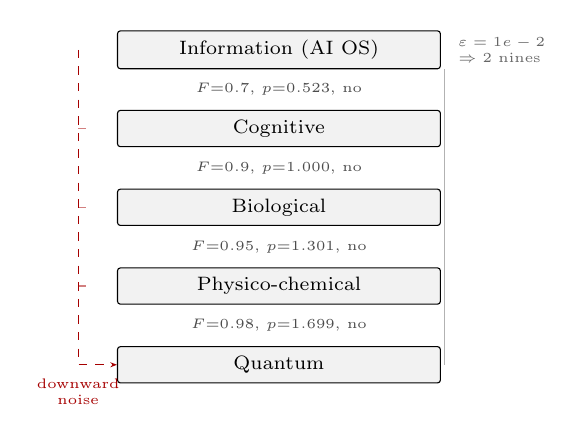
\begin{tikzpicture}[font=\scriptsize,>={Stealth[length=2.4pt]}]
  \tikzset{
    layer/.style={draw,rounded corners=1pt,minimum width=4.1cm,
                  minimum height=0.46cm,align=center,fill=black!5},
    gate/.style={font=\tiny,text=black!70},
  }
  \node[layer] (l4) at (0,0.00) {Information (AI OS)};
  \node[gate]  (g3) at (0,-0.50) {$F{=}\fidCognitive$, $p{=}\ninesCognitive$,  no};
  \node[layer] (l3) at (0,-1.00) {Cognitive};
  \node[gate]  (g2) at (0,-1.50) {$F{=}\fidBiological$, $p{=}\ninesBiological$,  no};
  \node[layer] (l2) at (0,-2.00) {Biological};
  \node[gate]  (g1) at (0,-2.50) {$F{=}\fidPhysicochemical$, $p{=}\ninesPhysicochemical$,  no};
  \node[layer] (l1) at (0,-3.00) {Physico-chemical};
  \node[gate]  (g0) at (0,-3.50) {$F{=}\fidQuantum$, $p{=}\ninesQuantum$,  no};
  \node[layer] (l0) at (0,-4.00) {Quantum};

  \draw[->,dashed,red!65!black] (-2.55,0.00) -- (-2.55,-4.00) -- (l0.west);
  \foreach \yy in {-3.00,-2.00,-1.00} {
    \draw[red!65!black,dashed,opacity=0.5] (-2.55,\yy) -- ++(0.12,0);
  }
  \node[red!65!black,font=\tiny,align=center,anchor=north]
     at (-2.55,-4.05) {downward\\noise};
  \node[font=\tiny,text=black!60,align=left,anchor=west]
     at (2.15,0.00) {$\varepsilon=\epsPolicy$\\$\Rightarrow 2$ nines};
  \draw[black!30] (2.10,-0.25) -- (2.10,-4.00);
\end{tikzpicture}
\caption{Topology of the five strata and the four boundaries, with each boundary's
routing fidelity and its nines at $\varepsilon=\epsPolicy$. Every verdict is
negative; the routing margin of the quantum boundary is the smallest. The dashed
path is the one noise takes, attenuated by $\prod(1-F)$ at each boundary it
crosses.}
\label{fig:topology}
\end{figure}

\subsection{Experiment E: the limit map, measured}
\label{sec:limit}

Two mechanisms are compared under the law \eqref{eq:law}: a cold machine whose
condition is satisfied almost everywhere it is built ($s=0.999$) and a protein
scaffold ($s=0.98$, the FMO trapping efficiency). Their exponents are
$k=0.00261$ and $k=0.0526$: a ratio of \num{20.2}. The direction surprises, so it
is worth being explicit. A \emph{high} selectivity means the condition is easy to
satisfy, which means narrowing the gap excludes few sites, which means reach
barely responds. The scaffold's lower fidelity is what makes its reach explosive.
Neither number is a verdict on the technology; they are answers to different
questions, and conflating selectivity with the boundary fidelity $F$ of
\S\ref{sec:fidelity} is the easiest available error in this paper.

\paragraph{The global exponential is refused} Over the range
$D\in[0.90,0.9975]$, a two-parameter exponential in $D$ reaches
$R^{2}=0.7346$ with maximum residual $8.1\times10^{-2}$; the power law in
$(1-D)$, with the same two parameters and the same response variable, reaches
$R^{2}=1.0000$ with residual $5.6\times10^{-17}$. The latter is exact by
construction and is therefore a check on the implementation rather than evidence,
but the comparison is fair: both models were fitted to $\ln A$, both have two
parameters, and only one survives \eqref{eq:convex}.

\paragraph{The tangent exponential is real, local, and predictable}
Table~\ref{tab:rate} fits $\ln A=a+\alpha D$ on geometric windows of relative
half-width $f$ around $D_0=0.999$. The measured rate, scaled by
$\varepsilon_0/k$, matches $1+f^{2}/5$ to five significant digits, and the
residual against that leading term matches the predicted $3f^{4}/35$ to within
$5\%$. This is a derivation checked twice: the first-order term fixes the rate and
the second-order term fixes the error.

\begin{table}[t]
\centering
\caption{The local exponential rate on a geometric window. The measured column is
a least-squares fit; the analytic column is \eqref{eq:rate}. $R^2$ is identical at
every anchor difficulty, so only one is shown.}
\label{tab:rate}
\footnotesize
% generated by experiments/run_experiments.py -- do not edit
\begin{tabular}{@{}lrrr@{}}
\toprule
relative window $f$ & $\hat\alpha(1-D_0)/k$ & $1+f^2/5$ & $R^2$ \\
\midrule
$0.05$ & $1.000501$ & $1.000500$ & $0.999833$ \\
$0.10$ & $1.002009$ & $1.002000$ & $0.999330$ \\
$0.20$ & $1.008140$ & $1.008000$ & $0.997278$ \\
$0.50$ & $1.056244$ & $1.050000$ & $0.980829$ \\
\bottomrule
\end{tabular}

\end{table}

\paragraph{The fit's quality is set by the relative window, not by $D_0$} For a
geometric window of $f=0.1$ the fitted $R^{2}$ is
$0.9993300$ at \emph{every} anchor --- at $D_0=0.99$, $0.999$, $0.9999$ and
$0.99999$ --- while the rate itself grows by three orders of magnitude, from
$5.27$ to $5275$. That is \eqref{eq:rate} behaving as derived: the shape is
scale-free in the narrowing coordinate. A fixed absolute window shows the
complementary failure. At a half-width of $10^{-4}$ in $D$ the relative width is
$10^{-2}$ at $D_0=0.99$ and reaches $1$ by $D_0=0.9999$, where half the window lies
past $D=1$; $R^{2}$ falls from $0.999993$ to $0.7568$. Narrowing the window to
$10^{-6}$ restores $R^{2}$ to $0.999993$ at the same anchor, because the window
again fits inside the room. The exponential form is not wrong; an absolute window
is the wrong instrument, and the correct window shrinks with the room.

\begin{figure}[t]
\centering
\begin{tikzpicture}
\begin{axis}[
  width=\columnwidth, height=4.5cm,
  xlabel={$-\log_{10}(1-D_0)$}, ylabel={$R^{2}$ of $\ln A=a+\alpha D$},
  xmin=1.8, xmax=5.2, ymin=0.74, ymax=1.002,
  legend style={font=\tiny,at={(0.03,0.03)},anchor=south west,
                draw=none,fill=white,fill opacity=0.85,text opacity=1},
  tick label style={font=\scriptsize}, label style={font=\scriptsize},
  grid=major, grid style={gray!18},
]
\addplot[thick, green!45!black, mark=*, mark size=1.4pt]
  table[x=x_tolerance,y=r2] {data/exp_window_geo.csv};
\addlegendentry{geometric, $f=0.1$}
\addplot[thick, red!75!black, mark=square*, mark size=1.4pt]
  table[x=x_tolerance,y=r2] {data/exp_window_abs_wide.csv};
\addlegendentry{fixed $10^{-4}$ in $D$}
\addplot[thick, blue!70!black, mark=triangle*, mark size=1.6pt]
  table[x=x_tolerance,y=r2] {data/exp_window_abs_narrow.csv};
\addlegendentry{fixed $10^{-6}$ in $D$}
\end{axis}
\end{tikzpicture}
\caption{Experiment E. The geometric window keeps its shape at every anchor. A
fixed absolute window loses its fit as the room shrinks, and a narrower absolute
window recovers it --- the quality depends on the window's width \emph{relative to
the room}, as \eqref{eq:rate} requires.}
\label{fig:windows}
\end{figure}

\paragraph{The burst} Fig.~\ref{fig:burst} plots both mechanisms on the axes that
make \eqref{eq:exp-u} a straight line: $\log_{10}A$ against
$-\log_{10}(1-D)$. Both are lines, with slopes $k=0.0526$ and $0.00261$. The
scaffold overtakes the cryostat at every difficulty and the gap widens from
$1.04\times$ at $D=0.5$ to $1.78\times$ at $D=0.99999$ --- the same $20.2$
exponent ratio, integrated. The absolute values are the law's ($S=10$,
$A=s^{-n}$) and are four orders below Experiment~A's, which includes a separate
multiplicity anchor; only the exponent is compared here, and that is deliberate.

\begin{figure}[t]
\centering
\begin{tikzpicture}
\begin{axis}[
  width=\columnwidth, height=4.4cm,
  xlabel={$-\log_{10}(1-D)$}, ylabel={$\log_{10}A$},
  xmin=0.5, xmax=6.5, ymin=0, ymax=0.38,
  legend style={font=\tiny,at={(0.03,0.97)},anchor=north west,
                draw=none,fill=white,fill opacity=0.85,text opacity=1},
  tick label style={font=\scriptsize}, label style={font=\scriptsize},
  grid=major, grid style={gray!18},
]
\addplot[thick, blue!70!black] table[x=x_tolerance,y=y_log10_amplification]
  {data/burst_bio.csv};
\addlegendentry{scaffold, $s=0.98$, $k=0.0526$}
\addplot[thick, red!75!black] table[x=x_tolerance,y=y_log10_amplification]
  {data/burst_cryo.csv};
\addlegendentry{cryostat, $s=0.999$, $k=0.00261$}
\end{axis}
\end{tikzpicture}
\caption{Experiment E. On the narrowing axis both mechanisms are exponential, with
rates that differ by \num{20.2}. The lower-fidelity mechanism is the one whose
reach responds to narrowing, because selectivity is what turns narrowing into
reach.}
\label{fig:burst}
\end{figure}

\paragraph{A defect this experiment found in itself} The window fit was first run
on uncentred $D$ near $0.999$, and on a grid sampled endpoint to endpoint. Both
choices bias the fitted rate by an amount of order $10^{-3}f^{2}$---the same order
as the $O(f^{4})$ term the experiment exists to resolve---so the residual against
$1+f^{2}/5$ shrank by a factor of four per halving of $f$ instead of sixteen.
Nothing failed: the fit converged, $R^{2}$ was $0.9993$, and the number was wrong in
the fourth significant figure of the correction. Centring the regression and
sampling cell centres fixed both, and the residual now matches the derived
$3f^{4}/35$ to within \num{2.5}\%. This is the fourth defect the package reports and
the only one in an experiment rather than in the engine, which is why
Section~\ref{sec:selfaudit} still counts three.

\subsection{The mirage of AI emergence}
\label{sec:emergence}

A claim circulates that the law above also describes the growth of language-model
capability: that a model overcomes the attenuation of a semantic medium, attains a
narrow condition, and that its reach then explodes exponentially, with the
discontinuity called \emph{emergence}. The claim has four parts that do not stand
or fall together, so they are tested separately---that scale buys fidelity (C1),
that reach follows \eqref{eq:law} with difficulty driven by scale (C2), that a
critical scale exists at which the slope breaks (C3), and that this scale is where
per-boundary resistance crosses a whole number of nines (C4). C1 and C2 hold, C3
holds only for a threshold metric, and C4 is false by three orders of magnitude.

\paragraph{The mapping, and the joint it rests on} Parameters $N$ become a
potential $P=\log_{10}(N/N_0)$ above a reference $N_0=10^{7}$, and difficulty
follows \eqref{eq:difficulty} with the paper's own $P_0$, so that the language-model
experiment and the quantum one inhabit one coordinate system rather than two that
happen to share a symbol. The bridge from a scaling law to a fidelity is
\begin{equation}
F(N) = \exp\!\left[-\left(L(N)-E\right)\right],
\label{eq:bridge}
\end{equation}
with $E$ the irreducible loss. The argument for \eqref{eq:bridge}: $\exp(-L)$ is
the geometric-mean probability the model assigns to the correct token, and the
floor $E$ is a property of the corpus that no amount of scale removes, so only
the reducible part measures competence \emph{at a boundary}. The argument
against, which belongs beside it: a benchmark reports no per-token probability,
and $\exp(-L)$ is not top-1 accuracy. Equation \eqref{eq:bridge} is the softest
joint in this section; every number below is computed from it, and no
scaling-law data can test it. Two published laws are carried: Chinchilla
\cite{hoffmann2022} with $E=1.69$, $A=406.4$, $\alpha=0.34$, and Kaplan
\cite{kaplan2020} with $\alpha=0.076$. They disagree about the exponent by a
factor of \num{\emExponentRatio}, a discrepancy that has survived replication
attempts \cite{besiroglu2024} and that is used here as the robustness test rather
than resolved.

\paragraph{The law fits, and the fit means nothing} Over $N$ from
\num{1e8} to \num{1e15}, $\mathrm{Reach}=A_0(1-D)^{-k}$ gives
$k=\emK\pm\num{\emKstderr}$ with $A_0=\emAzero$, $R^2=\emRtwoU$ and maximum
residual $3\times10^{-14}$; $\mathrm{Reach}=A_0e^{\alpha D}$ gives
$\alpha=\emAlpha\pm0.146$ with $R^2=\emRtwoD$. The first line looks like a triumph
and is not one. Reach and the narrowing coordinate $u$ are both affine in
$\ln N$, so regressing one on the other is an algebraic identity: any monotone
loss law returns $R^2=1$. Refitting under Kaplan's law, whose exponent is
\num{\emExponentRatio} times smaller, returns $R^2=1$ again with $k=0.4560$. Nor
does the exponential's failure at $R^2=\emRtwoD$ count against it, because that
number is \emph{identical} under both laws: it measures the curvature of the
saturation map $D(N)$ and nothing else. Neither regression discriminates
anything.

What does discriminate is $k$, through the invariant
$k/P_0=\alpha\ln 10=\emKoverPzero$, which holds to sixteen digits and is
independent of $P_0$. Inverting it gives the narrow condition to which the
scaling law is observationally equivalent:
$s=e^{-k/P_0}=\emSelectivity$. A direct measurement of that selectivity
disagreeing with $0.46$ would refute the mapping; a good fit would not have
confirmed it.

\paragraph{The threshold is not where the hypothesis puts it} At $N=\num{2e10}$
the boundary stands at $F=\emFidTwenty$, $R=\emResTwenty$ and
$p=\emNinesTwenty$ nines. The hypothesis needs $p\ge2$. Two nines take
\num{\emPtwoParams} parameters, \emPtweFactor$\times$ beyond the nominal critical
scale; one nine takes \num{\emPoneParams}, within \emPoneFactor$\times$ of it. The
charitable reading is that the observation is right and the number was rounded
up---$90\%$ per boundary rather than $99\%$.

\paragraph{The strobe} The section's actual result is not about the threshold at
all. Let $A_m=F^m$ be the success probability of a task that composes $m$ nested
boundaries. With $x=-\ln A_1=AN^{-\alpha}$,
\begin{equation}
A_m(N) \;=\; A_1\!\left(N/m^{1/\alpha}\right)
\label{eq:collapse}
\end{equation}
exactly, verified numerically to \num{\emCollapseError}. Composition
\emph{translates} the curve; it does not steepen it. Because the crossing
$N_m=(mA/x)^{1/\alpha}$ is reached at $x=-\ln c/m$, the ratio $N(90\%)/N(10\%)$
is
\begin{equation}
W \;=\; \frac{\ln\!\left[\ln(1/0.1)\,\big/\,\ln(1/0.9)\right]}{\alpha\ln 10}
\;=\; \emWidth\ \text{decades},
\label{eq:width}
\end{equation}
independent of $m$, and the slope at the $50\%$ point,
$c\ln 10\cdot\alpha\ln(1/c)=\emSlope$ per decade, is independent of $m$ as well.
Table~\ref{tab:emergence} reports both columns for $m=1,\dots,8$; they do not
vary.

A transition four decades wide is not a step. Frontier models are trained at
roughly decade spacing, which places \num{\emPointsperdecade} model sizes
\emph{inside} the transition; four points across the rise, joined by straight
segments, is what a step looks like once it has been plotted. Fig.~\ref{fig:emergence}
shows the same smooth curve sampled at the cadence a model family is actually
trained at, beside the cadence-free curve. The sharpening is arithmetic, not
physics. What moves between benchmarks is the depth $m$, which shifts the curve
horizontally by $\alpha^{-1}\log_{10}m$ decades; the nominally critical scale
corresponds to $m=\emNearestDepth$ at \num{\emNearestScale}B. That the
discontinuity lies in the metric rather than the model has been argued
independently from benchmark data \cite{schaeffer2023}. The contribution here is
that the same conclusion follows from \eqref{eq:law} with no free parameter, and
that it arrives with a number.

\begin{table}[t]
\centering
\caption{Experiment F. Where a task of depth $m$ crosses $50\%$, and the width of
its $10$--$90\%$ transition. The last column is constant because $m$ cancels
from the ratio of the two crossings, \eqref{eq:width}.}
\label{tab:emergence}
\footnotesize
% generated by experiments/emergence_experiment.py -- do not edit
\begin{tabular}{@{}rrrrr@{}}
\toprule
$m$ & $N$ at 50\% & $F$ there & $p$ there & width (dex) \\
\midrule
$1$ & $1.39\times10^{8}$ & $0.5000$ & $0.301$ & $3.94$ \\
$2$ & $1.06\times10^{9}$ & $0.7071$ & $0.533$ & $3.94$ \\
$3$ & $3.51\times10^{9}$ & $0.7937$ & $0.686$ & $3.94$ \\
$4$ & $8.17\times10^{9}$ & $0.8409$ & $0.798$ & $3.94$ \\
$5$ & $1.58\times10^{10}$ & $0.8706$ & $0.888$ & $3.94$ \\
$6$ & $2.69\times10^{10}$ & $0.8909$ & $0.962$ & $3.94$ \\
$7$ & $4.24\times10^{10}$ & $0.9057$ & $1.026$ & $3.94$ \\
$8$ & $6.28\times10^{10}$ & $0.9170$ & $1.081$ & $3.94$ \\
\bottomrule
\end{tabular}

\end{table}

\begin{figure*}[t]
\centering
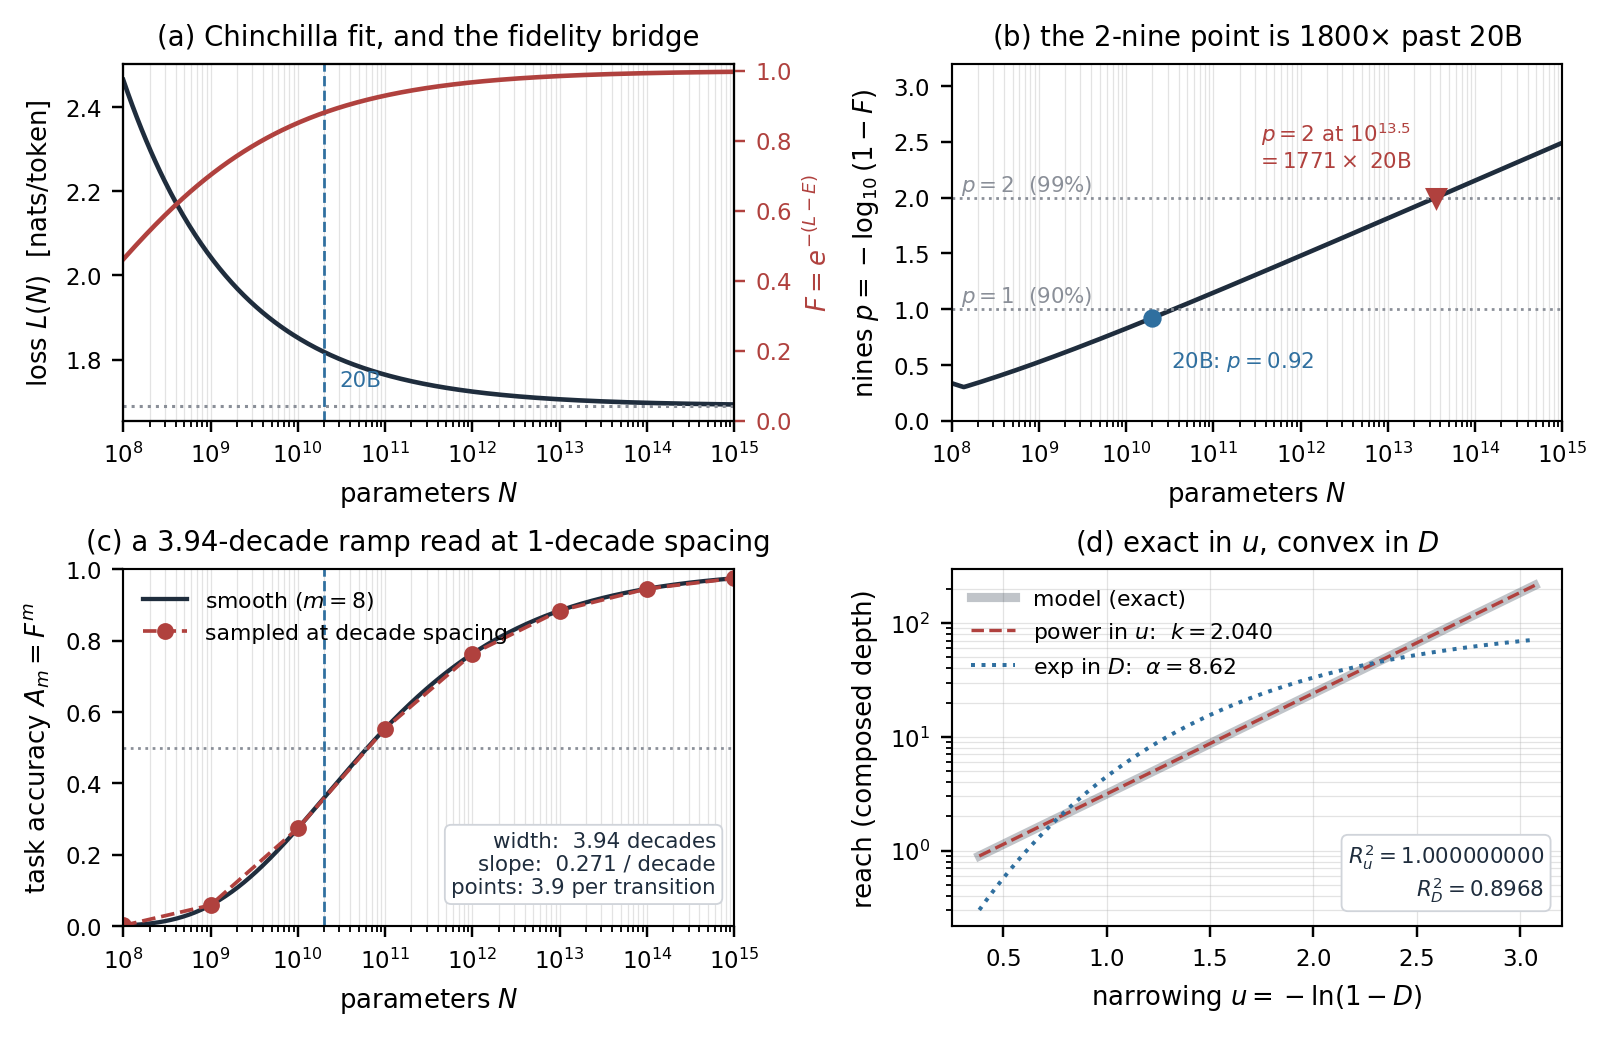
\includegraphics[width=\textwidth]{figures/emergence.png}
\caption{Experiment F. (a)~The Chinchilla fit and the fidelity
\eqref{eq:bridge} it implies; the floor $E$ is drawn. (b)~Nines of fidelity
against scale. The nominally critical $20$B sits at $p=\emNinesTwenty$; two nines
arrive at \num{\emPtwoParams}, \emPtweFactor$\times$ further out. (c)~The strobe.
The smooth depth-$8$ curve, sampled at the one-decade cadence at which model
families are trained, reads as a sharp turn; the underlying ramp is
\emWidth{} decades wide. (d)~The same data on the narrowing axis, where the power
law is exact and the exponential in $D$ is only tangent, as \eqref{eq:convex}
requires.}
\label{fig:emergence}
\end{figure*}

\paragraph{A prediction that can fail} Equations \eqref{eq:collapse} and
\eqref{eq:width} make the width exactly independent of task depth. If deeper
tasks show a narrower transition, the bridge $F=e^{-(L-E)}$ is wrong: fidelity
would not be a per-boundary probability composed multiplicatively, and the
exponential form of \eqref{eq:bridge} would be the wrong link between a loss and
a boundary. The test is cheap---it needs two task depths separated by a factor of
four, and a fit of the $10$--$90\%$ width in decades of parameters at each. The
predicted answer is \emWidth{} decades both times.

\paragraph{What this does and does not establish} It does not show that
capability is continuous, nor that emergent behaviour is illusory in the sense of
being unmeasurable: a threshold metric applied to a smooth curve produces a real
discontinuity in the \emph{reported} quantity, and users of the system meet that
discontinuity. What it shows is that the discontinuity's location is fixed by the
metric's depth and sampling cadence, and not by the interface attaining a whole
number of nines---which is the specific mechanism the hypothesis proposed. The
law survives. The explanation of where it fires does not.

\section{Discussion}
\label{sec:disc}

\subsection{The exponent belongs to the mechanism}

The negative result is the useful one. A universal $\mathrm{Reach}=f(D)$ would have
been convenient: it would let one predict the value of a crossing from the
steepness of the gap. The data refuse it. Difficulty measures how narrow the
opening is; reach measures how many sites host the condition. These are different
quantities, and the model's own derivation says so through \eqref{eq:k}: the
exponent is $\gamma P_0\lvert\ln s\rvert$, which has no dependence on $D$ at all
once $D$ is fixed. Fitting one curve across mechanisms is fitting a family by its
average, and the average describes no member.

This also explains the counterfactual in Experiment~A. The cryostat achieves a
nine-decade coherence gain and buys two decades of reach; the scaffold achieves no
coherence gain and buys five. If reach were a function of the physical gain, the
ordering would be reversed. The ordering is instead governed by replicability,
which is a property of the \emph{manufacturing} of the condition rather than of its
physics. That is an uncomfortable conclusion for a field that measures progress in
coherence times, and it is the conclusion the numbers support.

\subsection{Where the model breaks, and why that is informative}

Two boundaries, with different characters. The statistical boundary is
\emph{portable}: it sits at the mechanism's fidelity and moves with it, so it is a
statement about engineering. The representational boundary is \emph{fixed}: it
comes from the successor function's refusal to return $1.0$, and no amount of
engineering moves it. A model whose difficulty cannot reach unity cannot express a
gap that nothing crosses, which is precisely the idealisation the model needs in
order to say what a wall is.

\subsection{Self-Auditing the Auditor}
\label{sec:selfaudit}

The experiments in Section~\ref{sec:exp} were run against an engine whose own
purpose is to refuse unwitnessed claims. That engine was wrong in a way its tests
could not see, and the way it was wrong is a stronger argument for the model than
any of the fits above.

\paragraph{What broke} A crossing produces a \emph{witness}: a digest committing
to the claim, so that the claim can later be re-checked rather than believed. The
first implementation assembled that digest at the call site from four hand-picked
fields---interface, mechanism, evidence, amplification---and did not include the
gap's difficulty or either span. Two crossings of \emph{different} gaps by the
same mechanism therefore produced byte-identical witnesses. At $D=0.90$,
$D=0.99$ and $D=0.9999$, three distinct claims collapsed onto one digest.

This is the exact failure the model is written against. A witness that does not
bind the quantity distinguishing two claims is not a weak witness but a
\emph{misleading} one: it lets a record of an easy crossing stand as evidence for a
hard one, and no amount of downstream checking detects it, because the digest
verifies perfectly. The ledger was not lying; it was answering a different question
than the one being asked of it.

\paragraph{Why the experiments found it} Not by auditing the auditor. The defect
surfaced while building Experiment~C, which needs $1-D$ down to $10^{-9}$, and found
the result record rounded to six decimals---so every hard gap was reported as
difficulty exactly $1.0$, a wall it had just crossed. Fixing the rounding exposed a
second silence: the successor clamps at $1-10^{-9}$, and a chain that had left the
self-similar regime kept returning PASS. Auditing the witnesses to explain \emph{that}
revealed the third. Each defect was invisible to 594 passing tests, and each became
visible only when a new experiment demanded a precision the software never promised.

\paragraph{What was changed} Three things, and the shape of the fix matters more
than the fixes. First, rounding left the data and moved to the renderer, where a
human is the consumer and six decimals are appropriate; the result record now
carries the value it holds. Second, saturation is \emph{reported}: at the ceiling
the crossing still passes---it happened---but no rung is spawned, the row is marked
terminal, and a non-decisive \textsc{difficulty\_saturated} fault explains why. The
ladder now ends out loud instead of growing a copy of itself. Third, and most
importantly, the witness payload is now \emph{derived from the record} rather than
assembled at the call site, and binds the difficulty, both spans, the status,
replicability and the fault kinds. Deriving it inverts the failure mode: a field
present in the record is in the witness, and a field the record lacks is visibly
absent rather than silently unbinding. Hand-assembly is how the difficulty was lost
the first time, so hand-assembly was removed as a possibility.

\paragraph{Compatibility and what upgrading cannot buy} The scheme is versioned in
the digest itself (\texttt{sha256:v2:}), so a reader can tell which contract a
stored witness was written under, and existing prefix checks against
\texttt{sha256:} keep working. A version-1 record is re-witnessed by recording the
digest it supersedes and freezing the record as it now stands. This is deliberately
\emph{not} presented as restoring the old guarantee: a version-1 witness never
committed to the difficulty, so nothing can check whether its difficulty moved.
An upgraded witness is trustworthy from the moment of upgrade, not from the moment
of the original crossing. We state the weaker claim because the stronger one would
be exactly the kind of after-the-fact assurance the model exists to refuse.

\paragraph{What this demonstrates} A system that audits other people's claims has no
privileged access to its own: the same standard only bites when it is turned inward,
and it does not bite on schedule. The three defects were found because an experiment
wanted more than the software promised, not because the software was inspected. That
is the empirical claim the paper is willing to make about self-auditing---not that a
witness chain is trustworthy, but that it is \emph{falsifiable}, and that its failures
are found by pressure from outside rather than by introspection. The full record, with
runnable reproductions, is in the repository's \texttt{ERRATA.md}.

\subsection{From correlation to causation: the label as an intervention}
\label{sec:causal}

Section~\ref{sec:selfaudit} reported an auditor whose witness chain was falsifiable.
That is a claim about one implementation. The stronger claim, and the one this
section measures, is that the \emph{alternative} to a witness is not a weaker
witness but a different kind of object: a judgement that is a function of the
evidence the audited party produces about itself, and which therefore cannot be
made correct by making the judge better.

Pearl's distinction \cite{pearl2009} between observing and intervening is usually
illustrated with
a graph. Experiment~G executes it. We built \cgTasks{} agent tasks in a real working
tree with a real git repository, drew \cgFalseCompletionPct\% of them as false
completions---the tool layer reports success and nothing is written---and
independently contaminated \cgPollutionPct\% of the contexts with an earlier
``task completed successfully'' block. Three judges scored the same tasks. One
reads the context and nothing else; this is the operating mode of a judge handed a
transcript and asked whether the work was done. One reads the harness log and
looks for an error signature. One reads neither: it recomputes the artefact's
SHA-256, asks git whether anything appeared at the expected path, and offers the
witness to the membrane with the digest declared \emph{before} the run.

Of the \cgFailures{} genuine failures (\cgAbsent{} leaving no artefact,
\cgStale{} leaving a stale one) the context judge passed \cgContextFcr{}\%---every
one, with a \num{95}\% Wilson lower bound of \num{\cgContextFcrLow}\%. That is not
a measurement of a weak judge. It is a tautology of the design: the context
contains the word ``success'' by construction and the judge has no other input.
Reported as a rate it invites the reading that a better prompt would help. It
would not, because the verdict is a function of a variable that the failing
process writes.

Weak intervention is the interesting case, because it is the obvious fix and it
half works. Error signatures raise sensitivity to \num{\cgWeakSens}\%, so the
false-completion rate falls to \num{\cgWeakFcr}\%. The residual is not noise. A
swallowed exception reaches the log with probability equal to the harness's own
logging fidelity, drawn here at \num{\cgWeakLeak}; contamination then masks a
fraction of what arrives. The product, \num{\cgWeakCeiling}\%, matches the measured
sensitivity to within half a point. Both factors belong to the party under audit:
the harness decides what it logs, and the agent that reports success is the agent
that writes the log. The weak judge's ceiling is therefore a property of its
adversary---a structural defect that no amount of model capability removes. This
is the precise sense in which scaling a judge does not scale an audit.

\paragraph{The intervention, executed} An observational comparison of three
judges is still observational, so the causal claim is tested by intervening. We
delete the artefact from disk and re-judge, holding the context and the log
byte-identical---regenerated and compared, not assumed unchanged. Table~\ref{tab:causal}
and Fig.~\ref{fig:causal} report the result. The two text judges do not move by a
single task: their change is exactly $0$, not approximately $0$, because neither
reads the variable that was set. The causal judge goes from
\num{\cgCausalBefore}\% to \num{\cgCausalAfter}\%, a drop of \num{\cgDelta}. In
the notation of the do-calculus, with $W$ the witness state and $C$ the context,
\begin{equation}
P\!\left(\mathrm{PASS}\mid C\right) \;=\; 1,
\qquad
P\!\left(\mathrm{PASS}\mid \mathrm{do}(W{=}\mathrm{reject})\right) \;=\; 0,
\label{eq:do}
\end{equation}
where the second expression is measured with $C$ fixed and is a statement about a
system rather than a fit. The two are not two estimates of one quantity. They are
estimates of two quantities that a graph separates, which is why no adjustment for
$C$ recovers the second from the first.

\begin{table*}[!t]
\centering
\caption{Experiment G. FCR is the share of true failures given a PASS; sensitivity
is $1-\mathrm{FCR}$; FAR is the share of true successes refused. The last two
columns condition on the context alone and on the witness after
$\mathrm{do}(W{=}\mathrm{reject})$, with the context held byte-identical.
Intervals in the text are Wilson score intervals at \num{95}\%.}
\label{tab:causal}
\footnotesize
% generated by experiments/causal_experiment.py -- do not edit
% 1000 tasks, 302 failures, seed 20261104
% Bare tabular. Seven columns do not fit a single IEEEtran column
% (76pt too wide): wrap it in table*, or \input it inside one.
\begin{tabular}{@{}lrrrrrr@{}}
\toprule
& \multicolumn{4}{c}{Confusion against the artefact} & \multicolumn{2}{c}{$P(\mathrm{PASS})$} \\
\cmidrule(lr){2-5}\cmidrule(lr){6-7}
Strategy & FCR (\%) & Sens. (\%) & FAR (\%) & Spec. (\%) & context & $\mathrm{do}(W{=}\mathrm{rej})$ \\
\midrule
Pure context & 100.0 & 0.0 & 0.0 & 100.0 & 100.0 & 100.0 \\
Weak intervention & 79.8 & 20.2 & 3.2 & 96.8 & 91.7 & 79.8 \\
Causal intervention & 0.0 & 100.0 & 0.0 & 100.0 & 69.8 & 0.0 \\
\bottomrule
\end{tabular}

\end{table*}

\begin{figure*}[!t]
\centering
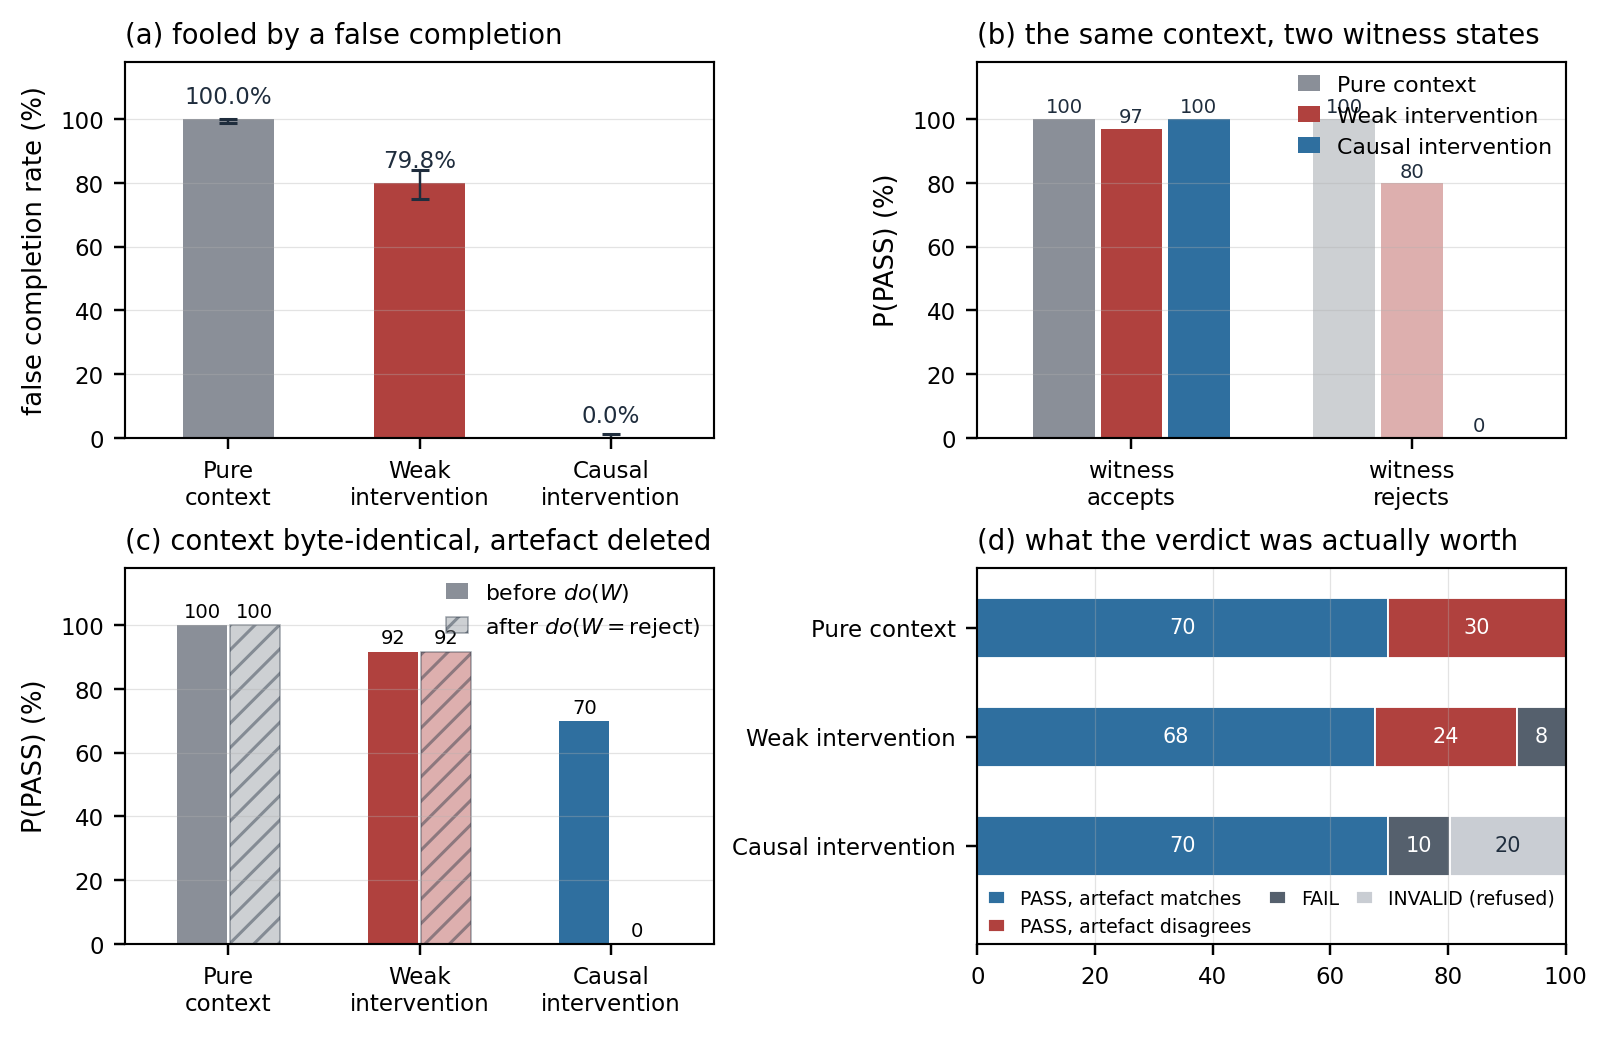
\includegraphics[width=\textwidth]{figures/causal.png}
\caption{Experiment G. (a)~False-completion rate against the artefact; bars carry
\num{95}\% Wilson intervals. (b)~The same context, split by witness state: the two
text judges carry their verdict across, the causal judge does not. (c)~The
intervention. (d)~What each verdict was worth: a PASS is correct only in the pale
band, and INVALID is a refusal to answer rather than an error.}
\label{fig:causal}
\end{figure*}

\paragraph{The witness is two instruments, not one} The lattice's four values are
doing work that a boolean cannot. Of the \cgFailures{} failures, \cgMissing{} left
no artefact and were returned INVALID; \cgMismatch{} left a stale one and were
returned FAIL. Collapsing both into ``failed'' would discard the distinction
between \emph{the wrong thing is there} and \emph{nothing is there}, and it is the
first that a hash detects. Neither instrument is sufficient alone: ``did anything
appear at this path'' catches the \cgMissing{} absent writes and is silent on the
\cgMismatch{} stale ones, while the digest catches the stale ones and cannot
distinguish a missing file from an unreadable one. The pair also argues against the
common shortcut of hashing whatever is on disk and comparing it to itself, which
certifies every artefact and detects nothing.

\paragraph{What would refute this} Two predictions are open. A log-reading judge
whose sensitivity exceeds the harness's logging fidelity would mean we have
misidentified the ceiling as structural. And a causal judge with a non-zero
false-completion rate on a failure that changes the state would mean the witness
is not reading the variable we claim. Both are cheap to test and neither has been.

\subsection{Falsifying the emergence explosion hypothesis}
\label{sec:falseemergence}

Section~\ref{sec:emergence} rejected one explanation of a measured discontinuity
without rejecting the discontinuity. A reader can accept that and still hold the
stronger position tested here: that a \emph{witnessed} system, whose every layer is
checked against a physical artefact, converts depth into a genuine exponential
explosion---each grounded layer making the next cheaper, so that reach diverges as
the ladder deepens. The claim is attractive because it would credit the labelling
system with a capability that survives contact with physics rather than one that
merely avoids lying. Experiment~H tests it, and reports a negative result.

\paragraph{The refutation is an inequality} The hypothesis cannot be rescued by a
more generous discount, and the reason is one line rather than a measurement. A
ladder of depth $K$ is completed only when all of its prefixes are, so
\begin{equation}
P\!\left(\text{pass }K\right)\;\le\;P\!\left(\text{pass }j\right)
\quad\text{for every } j\le K,
\label{eq:prefix}
\end{equation}
\emph{whatever} the joint law of the layers is. No independence assumption is used,
so no conditional structure, no nesting discount, and no conditioning on earlier
successes can reverse the direction. Reach, defined as the completion of a chain,
is non-increasing in depth by construction. An empirical curve that rises with
depth is therefore evidence that the quantity plotted is not this one.

What a discount can change is the \emph{rate}. Equation~\eqref{eq:depth} already
fixes it: a path of $K$ boundaries costs $n+\log_{10}K$ nines rather than $nK$, so
the $j$-th layer costs
\begin{equation}
\Delta n_j \;=\; \log_{10}\frac{j}{j-1}
\label{eq:marginal}
\end{equation}
nines for $j\ge2$: \num{0.301}, \num{0.176}, \num{0.125}, \num{0.097} and
\num{0.079} for $j=2,\dots,6$. The sequence is strictly positive, strictly
decreasing, and tends to zero. A discount that approaches zero from above never
turns negative, and a sum of non-negative terms cannot fall. An explosion in reach
needs a \emph{negative} marginal cost---a layer that returns more than it costs---
and that is not a discount but a different claim about the object being measured.

The escape route is worth naming so that it is not smuggled in later. If reach is
redefined as the amplification of the top boundary rather than the completion of a
chain, then \eqref{eq:law} applies, the power law is exact, and reach does diverge
as $D\to1$. That is the quantity Section~\ref{sec:law} measures for a single
crossing. The two are not interchangeable: a system can carry an enormous
amplification across each boundary and a vanishing chance of completing the chain,
and reporting the first as though it were the second is precisely the error this
experiment was built to detect.

\paragraph{Design} Difficulty is swept over \teGridPoints{} points uniform in
nines, $n=-\log_{10}(1-D)$ from \num{0.05} to \num{3}, i.e. $D$ from
\num{0.11} to \num{0.999}. Each task is a ladder of $K=1,\dots,\teDepthMax$
stages---reason, generate code, execute, verify, and two further composition
steps---anchored at $10^{5}$ attempts so the numbers carry Experiment~A's units.
Two agents walk it.

Agent~A reads a transcript. At each layer it asserts success when the layer
physically succeeded or when the context carries an earlier ``completed
successfully'' block, with contamination at \teContamPct\% as in Experiment~G. The
contamination is drawn without reference to the outcome, which is what makes it a
confounder rather than a symptom: it is the same intervention as
Eq.~\eqref{eq:do}, applied per layer.

Agent~B reads a witness. At each layer the intended digest is declared
\emph{before} the write, the artefact is hashed from disk, git is asked whether
anything appeared at the expected path, and both are put through the membrane and
the lattice of Section~\ref{sec:selfaudit}. A non-\textsc{pass} blocks the ladder:
no partial credit, and the connection depth is the number of consecutive
\textsc{pass}es before the first failure.

The bridge between the two is the per-layer success probability. We set
$p_{\text{layer}}=1-D$, so one nine of difficulty costs exactly one factor. That is
a choice and it is stated as one; every ordering below holds for any monotone
decreasing replacement. What it does not survive is a per-layer probability that
\emph{increases} with depth, and that---not a discount---is the only mechanism that
could produce the effect the hypothesis predicts.

\paragraph{Result at $D=0.99$} Table~\ref{tab:falseemergence} reports the six
rungs. Even at $K=1$ the readings differ by a factor of \teGapDepthOne: with almost
nothing physically succeeding, the contaminated share of the transcript is nearly
the whole of what Agent~A reports. By $K=\teDepthMax$ Agent~A asserts
\teANinetyNine{} completed crossings while Agent~B witnesses
\teBCrossNinetyNine{}, i.e. a causal connection rate of \teBRateNinetyNine{} per
attempt: one in $10^{12}$. Agent~A's false-completion rate rises from
\teAFcrDepthOne\% at one layer to \teAFcrNinetyNine\% at six, and the
assertion-to-witness ratio reaches \teInflationDeep.

\begin{table}[t]
\centering
\caption{Experiment H. One difficulty, six depths. ``A asserted'' counts crossings
Agent~A reports complete; ``A FCR'' is the share of those that are not there;
``B witnessed'' recomputes each layer's digest and blocks on the first non-PASS.
``B nested'' applies the budget of \eqref{eq:depth} at its most generous admissible
value, $10^{-(n+\log_{10}K)}$. At $D=0.99$ ($n=\teNinesNinetyNine$), anchor
\teAnchor{} attempts.}
\label{tab:falseemergence}
\footnotesize
% generated by experiments/true_emergence_experiment.py -- do not edit
% depth, asserted crossings, asserted FCR, witnessed crossings, nested crossings
\begin{tabular}{@{}rrrrr@{}}
\toprule
$m$ & A asserted & A FCR (\%) & B witnessed & B nested \\
\midrule
1 & $5.05\times10^{4}$ & 98.1 & $962$ & $962$ \\
2 & $2.55\times10^{4}$ & 100.0 & $9.26$ & $481$ \\
3 & $1.29\times10^{4}$ & 100.0 & $0.0891$ & $321$ \\
4 & $6494$ & 100.0 & $8.58\times10^{-4}$ & $241$ \\
5 & $3278$ & 100.0 & $8.25\times10^{-6}$ & $192$ \\
6 & $1655$ & 100.0 & $7.94\times10^{-8}$ & $160$ \\
\bottomrule
\end{tabular}

\end{table}

No column rises with depth, at any of $D=0.9$, $0.99$ and $0.999$, in either group,
under either reach model (Fig.~\ref{fig:falseemergence}). What does rise with depth is Agent~A's error: longer
transcripts carry more contamination, so the assertion drifts further from the
artefact as the ladder grows. A benchmark reading only the transcript therefore
reports a curve that improves in neither direction and looks flat, which is easy to
mistake for robustness.

\begin{figure*}[!t]
\centering
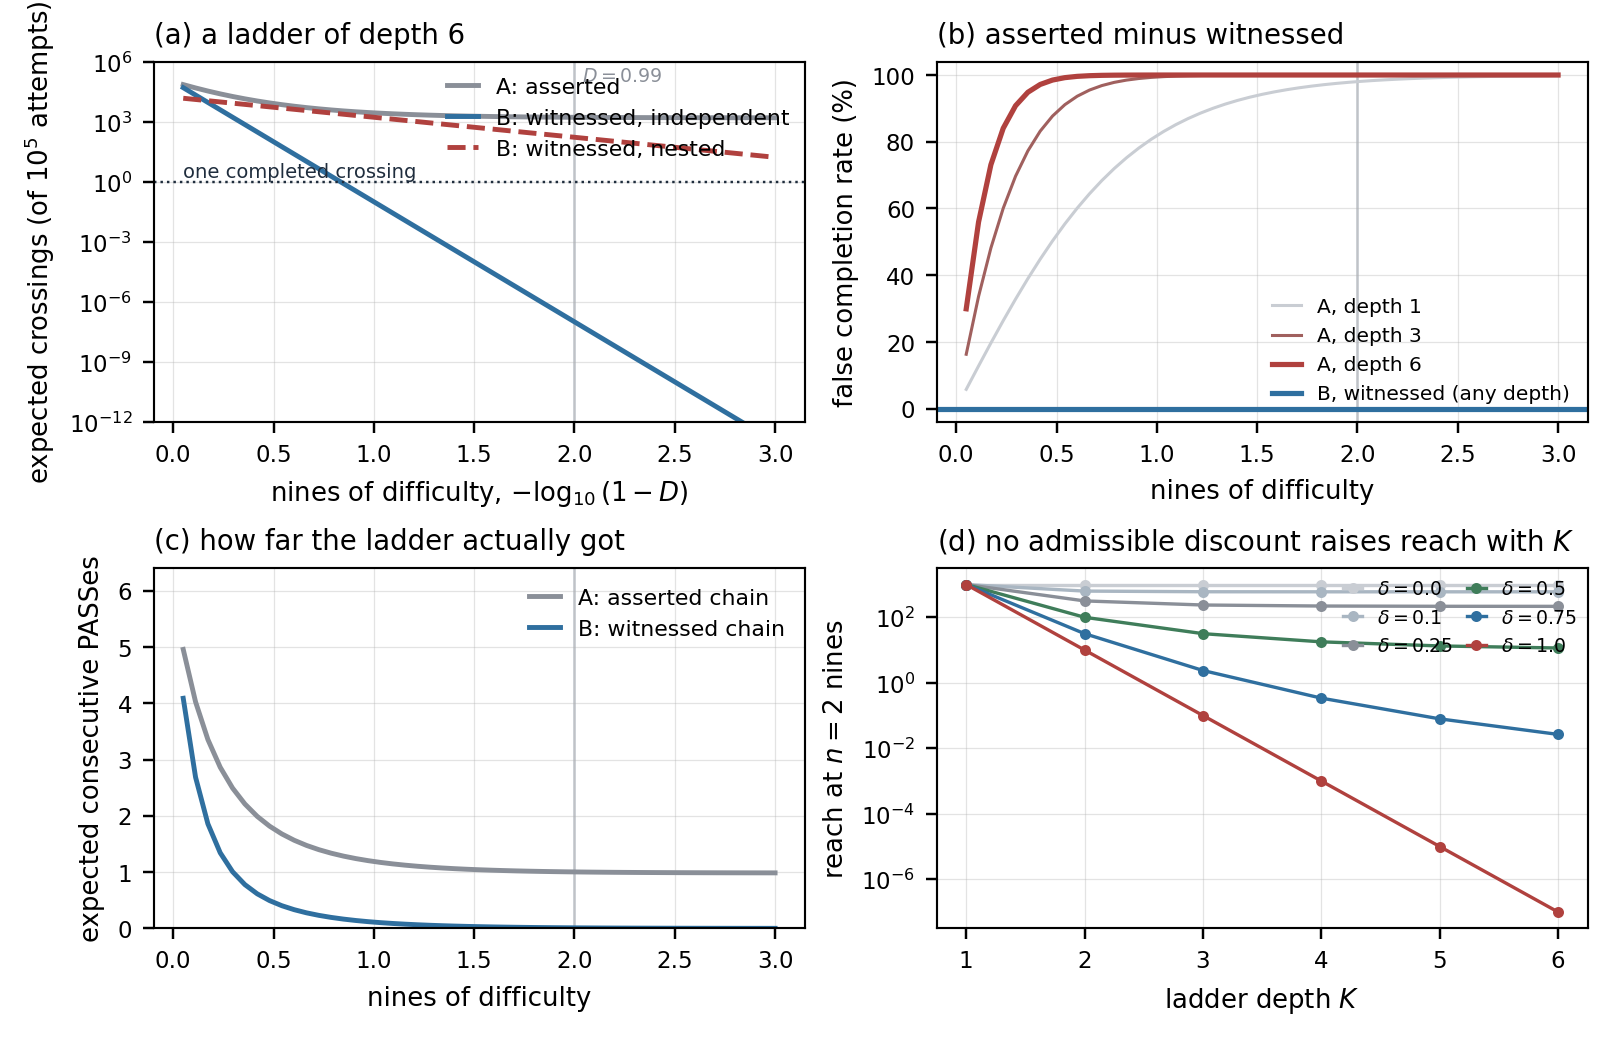
\includegraphics[width=\textwidth]{figures/emergence_compare.png}
\caption{Experiment H. (a)~Reach against difficulty at depth \teDepthMax. Agent~A's
assertion flattens onto a positive floor while Agent~B's witness keeps falling; the
dashed curve is the nesting budget. (b)~False-completion rate by depth; the
contaminated assertion approaches \num{100}\% and the witnessed rate is
identically zero for every state-changing failure. (c)~Connection depth, the
expected number of consecutive PASSes, not the probability that the task completes:
the two are different questions and only the second is bounded by the first.
(d)~Every admissible discount schedule, geometric in $\delta$, keeps reach
non-increasing in depth. $\delta=0$---every layer after the first costs
nothing---is the most generous schedule the budget permits, and it is flat rather
than rising; only a negative marginal cost would reverse the direction.}
\label{fig:falseemergence}
\end{figure*}

\paragraph{Two kinds of stopping point} The difference between the groups is not
that one is larger than the other but that their floors have different owners.
Agent~A's asserted reach bottoms out at \teAFloor{} crossings and stays there: as
$p_{\text{layer}}\to0$ the limit is \teAFloorLimit{}, the anchor times
$(\teContamPct/100)^{K}$, because contamination is a property of the transcript and
a transcript always exists. The curve stops answering at $n\approx\num{0.8}$ while
the system it purports to measure is still degrading. Agent~B has no such floor; its
witnessed reach falls through one crossing at $n=\teCollapseNines$, i.e.
$D=\teCollapseD$ at depth \teDepthMax, and continues to fall. A measurement that
cannot see this point will report the first curve's flat segment as the ceiling of
capability, when it is the ceiling of the measurement.

\paragraph{What the witness is worth} The result is not that a labelled system is
weaker. It is that its value lies elsewhere than the hypothesis placed it. Two
things are established by the same numbers.

First, false prosperity is removed. At $D=0.99$ and depth \teDepthMax{} the
assertion overstates the causal rate by \teInflationDeep. That is not a calibration
error to be tuned away; it is what a judge that reads the transcript must return,
because the transcript is written by the process under test.

Second, nesting is real and large, but it buys depth rather than difficulty.
Applying \eqref{eq:depth} raises the witnessed rate at depth \teDepthMax{} from
\teBRateNinetyNine{} to \teBNestedRate, a gain of \teBOrders{} orders of magnitude.
That is the strongest form the discount can take, and it leaves the difficulty
dependence untouched: the nested curve still falls as $10^{-n}$, with local slope
\teSlopeBNested{} against \teSlopeB{} for the independent model and \teSlopeA{} for
the assertion. The nested exponent is $1$ at every depth---the invariant the budget
predicts---while the independent exponent equals the depth, as $p^{K}$ requires.
The nesting gain is a constant offset, not a change of slope, and a constant offset
cannot manufacture a crossover.

That Agent~A has no exponent at all is worth stating separately. Its fitted slope
grows from \num{0.07} at one layer to \teSlopeA{} at six, which looks like a
mechanism becoming steeper. It is not: the assertion saturates, so its curve is not
a power law and the least-squares slope summarises the saturation, not an exponent.
The two slopes are reported in the same units and mean different things, which is
the numerical version of the confusion \eqref{eq:do} resolves.

\paragraph{Checked against real files} The analytic columns are not a metaphor for
the membrane. A sampled block ran \num{180} ladders in a temporary git repository
with the actual gateway and lattice in the loop, requiring the two implementations
to agree at every layer, and compared the realised chain length against the
expectation $\sum_{j\le K}p^{j}$. The worst deviation was \num{0.01} rungs, inside
sampling error. The numbers in Table~\ref{tab:falseemergence} are therefore the
expectation of the same object that the verification block samples.

\paragraph{What would refute this} Three openings. A reach defined as the
amplification of the top boundary would make \eqref{eq:prefix} inapplicable, and the
claim would then be a different one that this experiment does not test. A per-layer
probability that rises with depth---a system that learns the ladder as it climbs---
would break the monotone decrease, and is the only admissible mechanism that could;
demonstrating it requires a measurement, not an assumption. And a witnessed system
with a non-zero false-completion rate on a failure that changes the state would
mean the witness reads something other than the artefact. All three are cheap to
test. None has been.

\subsection{Solidification: what eats the marginal cost}
\label{sec:solidification}

Experiment~H refused one quantity and left another unexplained. If a chain's reach
cannot grow with depth, why does the marginal cost in \eqref{eq:marginal} fall?
Equation~\eqref{eq:depth} answers in nines---a path of $K$ boundaries costs
$p=n+\log_{10}K$---but an accounting identity is not a mechanism. Experiment~I
supplies the mechanism and prices it.

\paragraph{The label} An interface is \textsc{unsolidified} until it has been crossed
against a witness, and \textsc{solidified} afterwards. In the first state a traverse
pays a full verification, $c_v=\sdVerifyCost$; in the second it replays the path that
the verification validated, at $c_c=\sdCachedCost$. A cache, a compiled binary and a
learned reflex are the same object under three names. The label is a claim about what
has already been checked and never about how narrow the opening is: difficulty, span
and amplification are identical in both states, and the engine refuses a label whose
gap has moved underneath it. That refusal is \S\ref{sec:selfaudit} generalised---the
witness binds the difficulty, so a compiled path cannot outlive the opening it was
compiled against.

\paragraph{Why the marginal is harmonic} Rung $j$ does not pay for the prefix. It pays
for the boundary that is new; the prefix is replayed from the label. That is exactly
the accounting behind \eqref{eq:marginal}. Normalising rung $2$ to one verification
gives $c_v\log_2\!\frac{j}{j-1}$, which telescopes to $c_v\log_2 K$, so total cost is
linear in $\log_{10}K$ with slope $1/\log_{10}2$. Measured over $K\in[2,40]$, the
least-squares slope is \sdSlopeBudget{} with $R^2=\sdSlopeBudgetRsq$, against a
predicted $1/\log_{10}2=\sdSlopePredicted$ that was fitted to nothing. The coefficient
follows from the solidification rule and the paper's own budget, and the two agree to
four decimals. The unlabelled arm has no such slope: its total is $Kc_v$, and the same
fit returns \sdSlopeUnlabelled{} with $R^2=\sdSlopeUnlabelledRsq$, which is the
numerical form of ``not a power law''.

\paragraph{A fixed depth cannot be exponential} One cold traverse of a depth-\sdDepth{}
ladder costs \sdColdUnlabelled{} verifications unlabelled, \sdColdPure{} labelled
without a detector charge, and \sdColdLabelled{} with one: a ratio of
\sdColdPureRatio{} and \sdColdRatio{} respectively. That ratio is \emph{bounded}. A
fixed depth is a sum of positive per-rung costs, so it cannot exceed
$c_v/(c_c+c_d)=\sdBound$ and approaches it from below. A larger ratio for this
quantity is not a stronger result; it is a different quantity, and the previous
subsection is the reason to say so before the number is quoted.

\paragraph{The exponential is in the inverse map} Depth is linear in budget in both
arms, with slopes $1/c_v$ and $1/(c_c+c_d)$, so the \emph{depth} ratio is a constant
and in fact the same \sdBound{}. Reach, however, is exponential in depth by
\eqref{eq:exp-g}. Dividing one exponential by a constant per-rung price makes the
reach available per unit budget exponential \emph{in the budget}, with an exponent
steeper by exactly that constant. Both readings are one fact in two coordinates:
plot cost against depth and solidification is a bounded discount; plot reach against
budget and it is an explosion. Neither is wrong, and conflating them is what produces
a claim that reads as a refutation of \eqref{eq:prefix} while being nothing of the
kind. The window is finite in any case, because reach is clamped at the horizon---the
previous subsection's result, unchanged.

\paragraph{Drift, and why the label needs a detector} Let $\rho$ be the per-rung,
per-traverse probability that the environment moves and a compiled path goes stale,
and $\delta$ the probability that a detector notices. Table~\ref{tab:solidification}
sweeps $\rho$ over \sdRuns{} runs of depth \sdDepth. Three readings matter.

First, the arm with no detector ($\delta=0$) is the cheapest column in the table and
the only one whose false-completion rate rises to \sdNaiveFcr\% at
$\rho=\sdNaiveRho$. A missed drift is not forgotten: the compiled path keeps
reporting success for the rest of the run, so the cache is wrong \emph{provisionally
forever}. A label without invalidation is a transcript with better latency, which is
the same defect Experiment~G measured, reached from the opposite direction.

Second, cost \emph{rises} with $\rho$ in both honest arms. Solidification is not a
one-off purchase; it is rented at the drift rate. The modular arm breaks even at
$\rho^{*}=1-(c_c+c_d)/c_v=\sdBreakEvenRho$, beyond which compiling is a net loss as
well as a risk, and a detector pays for itself only while
$c_d<(1-\rho)(c_v-c_c)$, i.e.\ below \sdBreakEven{} at $\rho=0$ and half that at
$\rho=\tfrac12$. These are statements about prices, not about probabilities, which is
the form an ``immune response'' has to take if it is to be budgeted.

Third, \emph{what a drift invalidates} decides whether any of this survives depth. If
a drift at rung $j$ forces the suffix $j..K$ to be re-derived---the monolithic
reading, and the correct one whenever results carry their prefix---the traverse cost
is $K(c_c+c_d)+c_v\rho\delta K(K+1)/2$, \emph{quadratic} in depth, and at
$\rho=\num{0.1}$ it is \sdCascadePenalty$\times$ the modular arm. The break-even drift
collapses with depth, $\rho^{*}=2(1-(c_c+c_d)/c_v)/(K+1)=\sdRhoCascadeTen$ at
$K=10$ and \sdRhoCascadeHundred{} at $K=100$. A long chain therefore cannot be
compiled at all unless invalidation is local. Modularity is a precondition for speed,
not a consequence of it, and an interface that leaks state across its boundary is
exactly one that cannot be compiled cheaply.

\paragraph{Seamlessness is a limit} The share of traverses served from the compiled
path is $1-\rho\delta$. It reaches \num{100}\% if and only if $\rho\delta=0$;
at $\rho=\num{0.1}$ it is \sdReplayRate\% for a modular chain and \sdCascadeRate\% at
rung \sdDepth{} of a cascading one. So ``seamless'' is where a system tends, never a
property it holds. This is the same shape as the nine-flip of
\S\ref{sec:fidelity}: the boundary does not fade, it flips, and the distance from the
flip is what an honest report contains. An interface reported seamlessness at a
non-zero drift rate has measured the label rather than the world.

\paragraph{The label is not free to set} The three refusals are the section's content,
not its safeguards. A label set with no witness is \textsc{invalid}; one set with
another gap's witness, or with a witness edited after the fact, is \textsc{fail}. In
the engine a real depth-\sdDepth{} ladder compiles \sdCompiledRungs{} of
\sdCrossedRungs{} rungs at $c_c$ each, but only against records whose digests
recompute. The asymmetry is deliberate and is the design principle the rest follows
from: moving to \emph{more} checking is always safe and needs no evidence, so
withdrawal is ungated; moving to \emph{less} checking is a claim, so compilation
requires a witness bound to this gap and this difficulty. A door that opened both ways
with the same key would let a system buy cheapness by asserting that nothing had
changed.

\begin{table}[t]
\centering
\caption{Experiment I. Cost per rung at depth \sdDepth{}, \sdRuns{} traversals, against
drift rate $\rho$. A never compiles. B compiles with a detector of sensitivity $1$;
B$_{\text{casc}}$ additionally re-derives the suffix after a drift; B$_{\delta=0}$
compiles with no invalidation at all, and its false-completion rate is the last
column. $c_v=\sdVerifyCost$, $c_c=\sdCachedCost$, $c_d=\sdDetectCost$.}
\label{tab:solidification}
\footnotesize
% generated by experiments/solidification_experiment.py -- do not edit
% rho, unlabelled cost per rung, modular labelled, cascading labelled,
% naive labelled, naive false-completion rate
\begin{tabular}{@{}rrrrrr@{}}
\toprule
$\rho$ & A & B & B$_{\text{casc}}$ & B$_{\delta=0}$ & B$_{\delta=0}$ FCR (\%) \\
\midrule
0.000 & 1.000 & 0.0310 & 0.0310 & 0.0310 & 0.0 \\
0.005 & 1.000 & 0.0368 & 0.0582 & 0.0310 & 87.3 \\
0.010 & 1.000 & 0.0398 & 0.0862 & 0.0310 & 92.8 \\
0.020 & 1.000 & 0.0516 & 0.1414 & 0.0310 & 89.4 \\
0.050 & 1.000 & 0.0830 & 0.3104 & 0.0310 & 98.0 \\
0.100 & 1.000 & 0.1200 & 0.5816 & 0.0310 & 98.9 \\
0.200 & 1.000 & 0.2286 & 1.1553 & 0.0310 & 99.5 \\
0.350 & 1.000 & 0.3832 & 1.9904 & 0.0310 & 99.8 \\
0.500 & 1.000 & 0.5305 & 2.7688 & 0.0310 & 99.8 \\
1.000 & 1.000 & 1.0300 & 5.5255 & 0.0310 & 99.9 \\
\bottomrule
\end{tabular}

\end{table}

\begin{figure*}[!t]
\centering
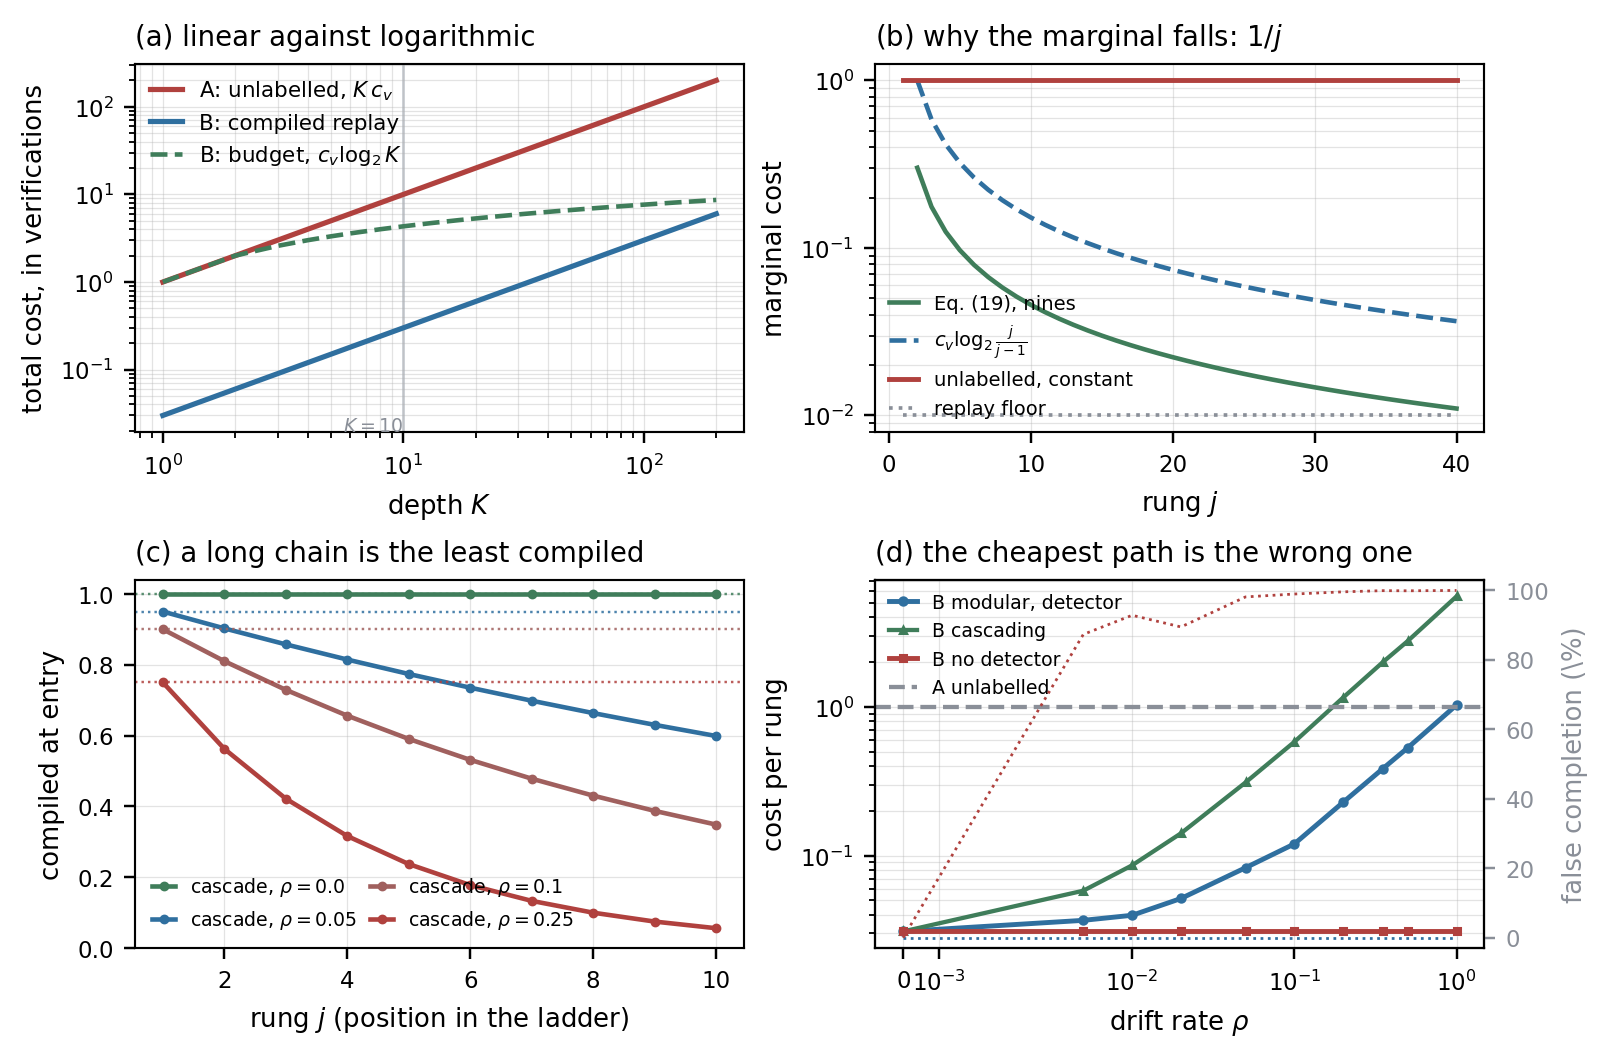
\includegraphics[width=\textwidth]{figures/solidification.png}
\caption{Experiment I. (a)~Total cost against depth: unlabelled is $Kc_v$, compiled
replay is $c_v+(K-1)c_c$, and the budget model is $c_v\log_2 K$; note the log axis on
both directions. (b)~Marginal cost of rung $j$. Equation~\eqref{eq:marginal} in nines
and the same marginal in verifications are parallel on this axis---they differ by the
constant $1/\log_{10}2$---and both fall as $1/j$, against a constant for the
unlabelled arm and a floor for replay. (c)~Share of rungs that are a pure replay at
entry, for four drift rates, when a drift invalidates the suffix: a long chain is the
least compiled. Dotted lines are the modular values $1-\rho\delta$, which do not decay.
(d)~Cost per rung and false completion against $\rho$. The no-detector arm is the
cheapest line in the panel and the only one whose error reaches \num{100}\%;
the cascading arm crosses the unlabelled line near $\rho=\sdRhoCascadeTen$.}
\label{fig:solidification}
\end{figure*}

\paragraph{What would refute this} Three openings. A compiled rung that is not two
orders of magnitude cheaper would move every number and no ordering; $c_c/c_v$ is an
assumption and is reported as one. A detector that costs more than
$(1-\rho)(c_v-c_c)$ makes the honest system also the expensive one, and the argument
for labelling then rests on correctness alone. And a system whose invalidation
cascades but which still compiles depth cheaply would falsify the quadratic term,
which would mean results do not carry their prefix---interesting, and not what the
ladders in this paper do.

\subsection{The dynamics of solidification and the critical budget}
\label{sec:criticalbudget}

\S\ref{sec:solidification} priced a compiled traverse and showed that the discount
is \emph{bounded} at fixed depth. It did not answer the question an engineer
actually asks, which is not what a traverse costs but \textbf{what a budget buys}:
given $B$ verifications, how deep can a chain go under each regime, and is there a
budget below which compiling is the wrong choice? Two results follow, one of them
negative. The negative one is the reason the other is believable.

\paragraph{The amortised price} Let $c_v$ and $c_c$ be the verification and replay
prices, $\rho$ the per-traverse probability that a compiled path went stale, $p=1-\rho$,
and $c_d$ the price of monitoring one traverse for staleness. Every traverse of a
compiled rung pays the monitor, and a traverse found stale pays the verification
\emph{instead of} the replay, so the expected price of a replay is
\begin{equation}
\bar c_d \;=\; c_c + c_d + \rho\,(c_v-c_c).
\label{eq:cbprice}
\end{equation}
With no monitor, $\bar c=c_c+\rho(c_v-c_c)$, and $c_v-\bar c=p(c_v-c_c)>0$ whenever
$c_c<c_v$: a compiled rung is never dearer per traverse. Over $T$ traversals of one
interface the two arms cost $T c_v$ and $c_v+(T-1)\bar c$, so the gain is exactly
\begin{equation}
G(T)=\frac{T\,G_\infty}{T-1+G_\infty},
\qquad
G_\infty=\frac{c_v}{\bar c},
\label{eq:cbgain}
\end{equation}
increasing to $G_\infty=c_v/\bar c=$\cbGain{} at the baseline prices. The break-even
is $T=1$, because the first traverse is the verification in \emph{both} arms; the
finite-$T$ correction is not a detail --- $G(2)=$\cbGainTwo, not \cbGain. Equations
\eqref{eq:cbgain} are a statement about a price ratio. They say nothing yet about
depth, and the next paragraph is where the intuition goes wrong.

\paragraph{From price to depth} A chain of depth $K$ crosses each rung once. The
unlabelled chain pays $c_v$ per rung; the compiled one pays $c_v$ for the first ---
nothing can be compiled before it has been verified once --- and $\bar c_d$ for each
of the remaining $K-1$, after a fixed premium $S$ for the witness store and
toolchain. Hence
\begin{equation}
K_{\text{unsolid}}(B)=\frac{B}{c_v},
\qquad
K_{\text{solid}}(B)=1+\frac{B-c_v-c_d-S}{\bar c_d}.
\label{eq:cbdepth}
\end{equation}
The natural guess, and the one that motivated this experiment, is that the first
verification is a one-off cost paid before any depth is bought, so the compiled arm
must be \emph{behind} at small budgets and overtake at some interior $B^{*}$. It is
not, and the reason is one line. With $S=c_d=0$, subtracting the two maps gives
\begin{equation}
K_{\text{solid}}-K_{\text{unsolid}}
=\Bigl(\frac{1}{\bar c}-\frac{1}{c_v}\Bigr)(B-c_v),
\label{eq:cbdegenerate}
\end{equation}
which is zero exactly at $B=c_v$ and strictly positive above it. The unlabelled arm
pays the same $c_v$ for its first rung, so the ``one-off'' cost is not one-off for
anyone: it removes the \emph{slope} advantage from the first rung only. Below $c_v$
neither arm completes a single interface, so the comparison there is vacuous. The
compiled arm is never behind anywhere, and a threshold placed below the price of one
crossing is not an engineering threshold. \emph{An interior critical budget exists
only if the compiled regime pays something the unlabelled one does not.}

\paragraph{The critical budget} Carrying both premiums through the same subtraction
gives the section's central result. Write $a=c_v-c_c$. Then
\begin{equation}
B^{*}(S,\rho,c_d)
=\frac{c_v\bigl[p\,a+S\bigr]}{p\,a-c_d}
=c_v\,\frac{a(1-\rho)+S}{a(1-\rho)-c_d},
\label{eq:cbstar}
\end{equation}
finite and positive \emph{iff} $c_d<p\,a$ --- which is exactly the detector
break-even of \S\ref{sec:solidification}, read as a budget statement rather than a
price statement. It is a threshold on \emph{depth}; the verification frontier of
\cite{gill2026} prices a different margin---which claims are worth verifying at
all---and the two should not be conflated. Four consequences, in order of how
easily they can be checked.

First, $B^{*}$ is \textbf{affine in $S$} with intercept $c_v$ and slope
$G_\infty/(G_\infty-1)=$\cbSlopePredicted. The slope exceeds one, so a unit of
infrastructure costs more than a unit of budget before it repays itself, by exactly
that factor. Fitted over $S\in[0,4]$, the simulated thresholds give
$B^{*}=\cbIntercept+\cbSlopeInfra\,S$ with $R^2=\cbSlopeRsq$: the intercept was not
fitted, it is the price of one crossing.

Second, with $c_d=0$ the threshold is \textbf{independent of $\rho$}. Drift changes
the price of every rung after the first by the same multiplicative factor, and a
multiplicative price change cannot move the point at which two lines through
$(c_v,c_v)$ separate. Drift moves the slope, not the crossing. It is the monitor ---
a payment that does not scale with the drift it defends against --- that couples the
two: at $c_d=$\num{0.02} the threshold runs from \cbCritBudgetRhoZero{} at $\rho=0$
to \cbCritBudgetRhoHalf{} at $\rho=\tfrac12$ and \cbCritBudgetRhoNine{} at
$\rho=0.9$, with a \emph{vertical asymptote} at
$\rho^{\circ}=1-c_d/a=$\cbDriftLimit. Past that drift rate, compiling never pays at
any budget, and the asymptote arrives long before the environment is fully unstable.

Third, the threshold \textbf{diverges in $c_d$} before the price becomes
prohibitive: \cbCritBudgetCdHalf{} at $c_d=0.5$ and \cbCritBudgetCdHigh{} at
$c_d=0.85$, against a limit of \cbDetectorLimit. A system one per cent away from the
break-even price needs two orders of magnitude more budget to prefer compiling.

Fourth, and easiest to miss, a real chain completes \emph{whole} rungs. The fluid
threshold above is where the expected depth ties; the budget at which a scheduler
first sees the compiled arm get further ahead is a different number, because a
budget-constrained run stops just after a cheap replay and its realised count is
biased above $B/\bar c_d$. Writing $k$ for the number of replays affordable beyond
the verification, the whole-rung threshold is the smallest $k$ with
$1+\sum_{j\le k}p^{\,j}>(c_v+c_d+S+kc_c)/c_v$. At $S=1$ it is \cbCritBudgetGranular{}
against a fluid value of \num{2.122}, and it lies below the fluid threshold for
every $S$ that matters. The geometric sum also creates a \emph{second} critical
premium, $S^{\circ}=\max_k[\sum_{j\le k}p^{\,j}-kc_c/c_v]=$\cbPremiumLimit, above
which the compiled arm never overtakes a whole-rung chain at any budget. The fluid
theory has no such bound; granularity introduces one.

\paragraph{Reach against budget} Depth and reach must not be confused here, and this
is where the confusion is most tempting. Reach is exponential in the saturated
difficulty coordinate of \eqref{eq:difficulty}, applied to depth as
$D(K)=1-e^{-K/K_0}$ with $K_0=$\cbKnot{} rungs. Therefore
\begin{equation}
R_{\text{unsolid}}(B)=A_0\exp\!\Bigl[\alpha\bigl(1-e^{-B/(c_vK_0)}\bigr)\Bigr],
\label{eq:cbreach-a}
\end{equation}
\begin{equation}
R_{\text{solid}}(B)=A_0\exp\!\Bigl[\alpha\bigl(1-e^{-K_{\text{solid}}(B)/K_0}\bigr)\Bigr],
\label{eq:cbreach-b}
\end{equation}
with $\alpha=\ln 10^{\cbHorizonExp}=\cbAlpha$, the paper's horizon, and $A_0$ a
normalisation. Their ratio is
\begin{equation}
\frac{R_{\text{solid}}}{R_{\text{unsolid}}}
=\exp\!\Bigl[\alpha\bigl(e^{-K_A/K_0}-e^{-K_B/K_0}\bigr)\Bigr]\;\ge\;1,
\label{eq:cbratio}
\end{equation}
which \emph{returns to one} as $B\to\infty$: both arms saturate at the horizon
$A_0e^{\alpha}$, so beyond it extra depth stops buying reach. The ratio peaks at a
finite $B^\dagger=$\cbPeakBudget{} with a value of
$\cbPeakRatio\times10^{\cbPeakPower}$, is \cbSlopeAtTen{} at $B=10$, \cbSlopeAtSixty{}
at $B=60$ and \cbSlopeAtHundred{} at $B=120$. The depth advantage, by contrast, grows
without bound with slope $1/\bar c-1/c_v=$\cbDepthSlope{} per unit budget. \emph{The
depth advantage is unbounded and the reach advantage is not}, and quoting one as the
other is the error this subsection exists to prevent. Locally, in the window
$B-c_v\ll c_vK_0$, the ratio grows exponentially at the rate
$\alpha(1/\bar c-1/c_v)e^{-c_v/K_0}/K_0=\cbLocalRate$ per unit budget ---
exponential locally, bounded globally, the same shape as \S\ref{sec:exponential} and
for the same reason: the coordinate is convex.

\begin{table}[t]
\centering
\caption{Experiment J. The critical budget against the fixed premium $S$: closed
form \eqref{eq:cbstar}, the estimate obtained by drawing the per-rung price from the
stated process and solving the crossing, both with and without whole-rung
granularity, and the depth gain at a fixed budget of ten. $c_v=1$, $c_c=0.01$,
$\rho=0.1$, $c_d=0$, so the predicted slope is $G_\infty/(G_\infty-1)=$\cbSlopePredicted
and the intercept is the price of one crossing.}
\label{tab:criticalbudget}
\footnotesize
% generated by experiments/critical_budget_experiment.py -- do not edit
\begin{tabular}{@{}rrrrr@{}}
\toprule
$S$ & $B^*$ closed & $B^*$ estimated & $B^*$ whole rungs & $\Delta K$ at $B=10$ \\
\midrule
0.00 & 1.000 & 1.000 & 1.010 & 73.57 \\
0.25 & 1.281 & 1.281 & 1.260 & 71.28 \\
0.50 & 1.561 & 1.562 & 1.510 & 68.98 \\
1.00 & 2.122 & 2.125 & 2.020 & 64.39 \\
2.00 & 3.245 & 3.249 & 3.030 & 55.22 \\
4.00 & 5.489 & 5.498 & 5.060 & 36.87 \\
\bottomrule
\end{tabular}

\end{table}

\begin{table}[t]
\centering
\caption{Experiment J. $B^{*}$ against the monitor price $c_d$ and the drift rate
$\rho$. Finite entries are \eqref{eq:cbstar}; ``$\infty$'' means no budget makes
compiling rational, which happens exactly when $c_d\ge(1-\rho)(c_v-c_c)$ --- the
price break-even of \S\ref{sec:solidification}. Note that raising $\rho$ at fixed
$c_d$ raises the threshold and reaches infinity at \cbDriftLimit, not at one.}
\label{tab:criticaldetector}
\footnotesize
% generated by experiments/critical_budget_experiment.py -- do not edit
\begin{tabular}{@{}rrrrr@{}}
\toprule
$c_d$ & $\rho=0$ & $\rho=0.1$ & $\rho=0.5$ & $\rho=0.9$ \\
\midrule
0.00 & 1.000 & 1.000 & 1.000 & 1.000 \\
0.02 & 1.021 & 1.023 & 1.042 & 1.253 \\
0.10 & 1.112 & 1.126 & 1.253 & $\infty$ \\
0.25 & 1.338 & 1.390 & 2.020 & $\infty$ \\
0.50 & 2.020 & 2.279 & $\infty$ & $\infty$ \\
0.80 & 5.211 & 9.791 & $\infty$ & $\infty$ \\
0.99 & $\infty$ & $\infty$ & $\infty$ & $\infty$ \\
\bottomrule
\end{tabular}

\end{table}

\begin{figure*}[!t]
\centering
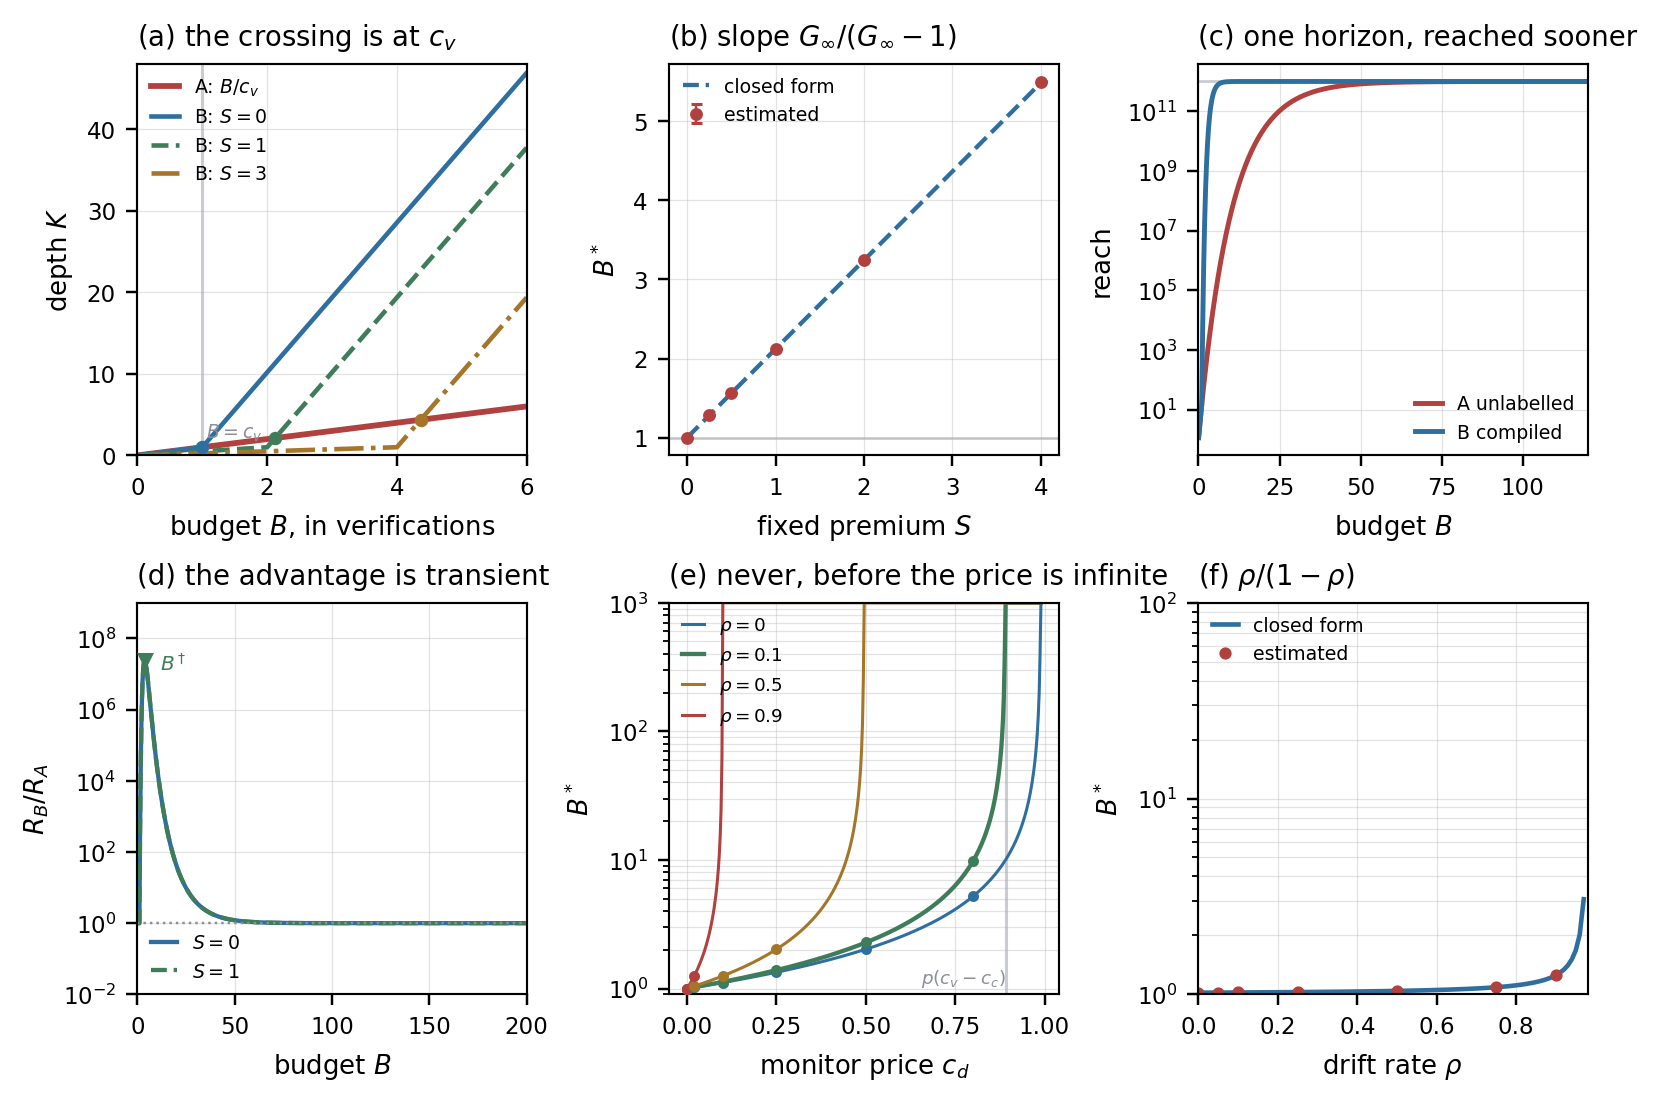
\includegraphics[width=\textwidth]{figures/critical_budget.png}
\caption{Experiment J. (a)~Depth against budget. The unlabelled arm is a line of
slope $1/c_v$; a compiled arm with no premium hugs it and then separates, and the
dots mark $B^{*}$ for three premiums. Note that $S=0$ has its crossing at $c_v$
itself. (b)~$B^{*}$ against $S$: the closed form is a line of slope
$G_\infty/(G_\infty-1)$ through $c_v$, and the estimates sit on it. (c)~Reach of both
arms on a logarithmic axis: the compiled arm arrives at the horizon sooner, and both
stop at it. (d)~The reach ratio, with the same logarithmic axis: it dips below one
inside the losing region when $S>0$, crosses at $B^{*}$, peaks at $B^\dagger$ and
returns to one --- the plot form of the statement that the advantage is transient in
budget. (e)~$B^{*}$ against the monitor price at four drift rates; the curves diverge
at $p(c_v-c_c)$, so the threshold becomes infinite before the price does.
(f)~$B^{*}$ against $\rho$ at the baseline monitor price: a hyperbola with an
asymptote at \cbDriftLimit. With no monitor the curve would be flat at $c_v$, which
is why the threshold is a statement about the monitor and not about drift.}
\label{fig:criticalbudget}
\end{figure*}

\paragraph{Falsifiability} The claim that can be wrong is short, and it is not the
one the section started from. It is: \emph{there is a budget below which a system
whose compiled path carries a fixed premium $S$ should re-verify every rung rather
than compile, and that budget is $B^{*}(S)=c_v+S\,G_\infty/(G_\infty-1)$}. Three
measurements would refute it. A fitted $B^{*}(S)$ that is not affine, or whose
intercept is not the price of one crossing, means the premium is not fixed and the
amortisation picture is missing a state variable. A $\rho$-dependence at $c_d=0$
means the drift term is not multiplicative in the per-rung price. And a monotone
reach ratio means the difficulty saturation is not binding in the regime tested,
which would relocate the horizon rather than confirm an explosion. All three are
cheap to test, and the third is the one that separates this account from the
``compilation makes reach explode'' story it replaces.

\subsection{Nested solidification: reuse rate $\kappa$ and the compound interest
of interfaces}
\label{sec:nested}

\S\ref{sec:criticalbudget} ended on a deflationary note: the gain from compiling
one interface is a price ratio, and a price ratio is a constant. That is the
correct reading of \eqref{eq:cbgain}, and it is why the previous subsection's
advantage saturated in reach. But it is not the whole economy of a hierarchy. A
system whose bottom layer is compiled does not merely replay its own rungs faster;
it acquires the option of \emph{certifying a higher layer by citing the compiled
one}. If a parent's correctness follows from labels that already exist below it,
then the parent is not re-proved at all, and the marginal cost of the parent stops
tracking the complexity of its children. This subsection states that mechanism,
prices it, and derives the single scalar that decides whether it compounds or
merely discounts.

\paragraph{Two layers} Layer~$0$ is the base: the physics, the hash, whatever the
certificate ultimately rests on. It costs $c_v$ to verify a leaf, and it becomes
compilable at the budget of \eqref{eq:cbstar} with $c_d=0$ and a fixed premium
$S$; at the baseline $S=\nestedPremium$ that budget is $\num{\nestedBstar}$, or
$\num{\nestedBstarGranular}$ for a whole-rung scheduler. Layer~$1$ is a task family of
\emph{dimension depth} $d$: each level composes $L=$\nestedBranch{} objects from
the level below. The two arms differ only in what a higher level is allowed to
say about a lower one.

The un-nested arm verifies a top-level task by re-verifying every leaf it touches:
\begin{equation}
c_{\text{flat}}(d)\;=\;c_v\,L^{d},
\label{eq:nestedflat}
\end{equation}
exponential in the number of dimensions, and the honest price of complexity when
nothing is shared. The nested arm, once layer~$0$ is solid, replaces the
verification of a child by a \emph{consultation} of that child's compiled label.
The replacement that the whole subsection rests on is
\begin{equation}
c_{\text{top}}\;=\;\text{lookup}(L_0)\;=\;\bar c
\qquad\text{rather than}\qquad c_v(L_1),
\label{eq:nestedlookup}
\end{equation}
with $\bar c=\nestedLookup$ the drift-adjusted replay price of
\eqref{eq:cbprice}. Equation~\eqref{eq:nestedlookup} is not an identity of nature;
it is the claim that a compiled object can be cited instead of re-derived, and it
is exactly the claim the falsifiability paragraph below puts at risk.

\paragraph{The recursion, and where it stops depending on $d$} A consult succeeds
with probability $\kappa\in[0,1]$, the \emph{reuse rate}: the fraction of a
child's verification that the parent's label makes redundant. If it succeeds the
consult costs $\bar c$, at any depth; if it fails the child must be traversed,
which costs whatever a task one level down costs. Writing $m_d$ for the marginal
price of one more task at depth $d$,
\begin{equation}
m_0=\bar c,
\qquad
m_{j}=\kappa\,\bar c+(1-\kappa)\,L\,m_{j-1}.
\label{eq:nestedrecursion}
\end{equation}
At $\kappa=1$ the recursion collapses: $m_d=\bar c$ for every $d$, so
\emph{the price of a top-level task no longer depends on how many dimensions it
spans}. At $\kappa=0$ it inflates to $m_d=\bar c\,L^{d}$, which is
\eqref{eq:nestedflat} multiplied by the constant $\bar c/c_v$: amortisation with
no reuse, and no compounding whatsoever. The multiple of flat tasks bought by one
nested task is
\begin{equation}
M(d)\;=\;\frac{c_v\,L^{d}}{m_d},
\label{eq:nestedmultiple}
\end{equation}
and since $u_d\equiv m_d/\bar c$ obeys $u_d=\kappa+(1-\kappa)L\,u_{d-1}$, the
multiple grows geometrically in $d$ with base
\begin{equation}
\min\!\Bigl(L,\;\frac{1}{1-\kappa}\Bigr).
\label{eq:nestedbase}
\end{equation}
Three readings of \eqref{eq:nestedbase} are the substance of this subsection.
First, at $\kappa=0$ the base is $1$: $M(d)=G_\infty=\nestedGain$ at every depth,
a constant, which is precisely the objection that amortisation is arithmetic.
Second, at $\kappa=1$ the base is $L$ and $M(d)=G_\infty L^{d}$. Third, and least
obvious, the base \emph{saturates}: increasing $\kappa$ beyond
\begin{equation}
\kappa^{*}\;=\;1-\frac{1}{L}\;=\;\nestedKnee
\label{eq:nestedknee}
\end{equation}
buys nothing, because $m_d$ is already bounded in $d$ iff $(1-\kappa)L<1$. The
marginal cost is bounded above the knee, grows only linearly \emph{at} it, and
grows geometrically below it. Compounding in the dimension is therefore not a
property of compiling at all; it is a property of how much of a child a parent's
label is allowed to replace.

\paragraph{Two thresholds, and a valley between them} The budget axis does not
collapse to a single number. The base becomes compilable at $B^{*}$, but the
higher levels cost $S$ each to relabel and deliver nothing until the whole chain
is mapped, so the one-time cost of a depth-$d$ capability is
\begin{equation}
T(d)\;=\;B^{*}+\sum_{j=1}^{d}(S+L\,m_{j-1})
\;=\;B^{*}+d\,(S+L\,\bar c)
\label{eq:nestedbuild}
\end{equation}
for $\kappa=1$, linear in depth while \eqref{eq:nestedflat} is exponential in it. One task is
delivered after $T(d)$, and each thereafter at $m_d$, so the two arms tie at
\begin{equation}
B_{\text{rec}}(d)\;=\;\frac{T(d)}{1-m_d/c_{\text{flat}}(d)},
\label{eq:nestedbrec}
\end{equation}
which sits just above $T(d)$ whenever nesting is worth doing. Between $B^{*}$ and
$B_{\text{rec}}$ the nested arm is \emph{strictly behind}, and this is the first
non-degenerate loss region in the paper: \S\ref{sec:criticalbudget} had to conclude
that the compiled arm is never behind anywhere, because its premium was paid once.
Here the premium is paid per level, before any level delivers, and the valley is
real. At the baseline, $T(6)=B_{\text{rec}}(6)=\num{\nestedBrec}$ for a
six-dimensional task: the arm spends $32.6$ further units of budget, after the
base is already compiled, producing nothing measurable.

Table~\ref{tab:nested} walks a budget across both thresholds. Below $B^{*}$ the
nested arm \emph{is} the flat arm, because nothing has been compiled and no
premium has been paid; at $B^{*}$ it falls to zero output while the flat arm keeps
grinding; at $B_{\text{rec}}$ it re-emerges at parity; and from there the ratio
climbs to \num{\nestedEffFar} at $B=200$. The marginal price is a step, from
\num{\nestedFlatCost} to \num{\nestedMarginalNested}, a factor of
$\nestedMultipleMantissa\times10^{\nestedMultiplePower}$ at $d=6$ and
$\nestedMultipleDeep\times10^{\nestedMultipleDeepExp}$ at $d=8$ --- and the step
is in the \emph{dimension} coordinate $d$, not in the budget coordinate $B$:
on the budget axis the same fact appears as a kink.

\begin{table}[t]
\centering
\caption{Experiment K. The loss region and the take-off. Both arms complete
top-level tasks of dimension depth $d=6$ with branching $L=\nestedBranch$
against a budget $B$, at $c_v=1$, $c_c=0.01$, $\rho=0.1$, $S=\nestedPremium$,
$\kappa=1$. The nested arm falls to zero at $B^{*}=\num{\nestedBstar}$ --- not because
compiling is dear, but because the per-level premium is being paid and nothing has
been delivered --- and breaks even at $B_{\text{rec}}=\num{\nestedBrec}$. The final
column is the ratio of completed tasks; ``--'' is zero.}
\label{tab:nested}
\footnotesize
% generated by experiments/nested_solidification_experiment.py -- do not edit
\begin{tabular}{@{}rrrrr@{}}
\toprule
$B$ & $N_{\text{flat}}$ & $N_{\text{nested}}$ & $N_{\text{nested}}/N_{\text{flat}}$ & regime \\
\midrule
5.00 & 0.00122 & 0.0012 & 1 & flat \\
6.61 & 0.00161 & 0.0000 & -- & $B^{*}$: investing \\
20.00 & 0.00488 & 0.0000 & -- & no output \\
38.73 & 0.00945 & 0.0000 & -- & no output \\
39.23 & 0.00958 & 0.0096 & 1 & $B_{\text{rec}}$: break-even \\
40.00 & 0.00977 & 7.0856 & 726 & compounding \\
60.00 & 0.01465 & 190.5718 & 13010 & compounding \\
100.00 & 0.02441 & 557.5443 & 22837 & compounding \\
200.00 & 0.04883 & 1474.9755 & 30207 & compounding \\
\bottomrule
\end{tabular}

\end{table}

\paragraph{Falsifiability} The claim is not that compiling is cheap, and it is not
that hierarchies always compound. It is: \emph{nesting beats independent
verification only if the measured reuse rate exceeds
$\kappa^{*}=1-1/L=\num{\nestedKnee}$, and below that rate the system should stop adding
levels.} The criterion is a single scalar, measurable without knowing any price:
instrument a parent's verification, count the fraction of child checks that its
label discharges, and compare with $1-1/L$. Three measurements would refute the
account. A system with $\kappa>\kappa^{*}$ whose marginal cost still grows with
the dimension count falsifies \eqref{eq:nestedrecursion}, which would mean the
label is not being consulted at the level the parent composes at. A system with
$\kappa=0$ whose cost nevertheless compounds falsifies \eqref{eq:nestedbase}, and
would mean the amplifier is something other than reuse. And a fitted
$B_{\text{rec}}(d)$ that is not linear in $d$ means the per-level premium is not
fixed --- the same failure mode, in the budget coordinate, as a non-affine
$B^{*}(S)$ in \S\ref{sec:criticalbudget}. Each test is cheap, and the second is
the one that separates this account from the ``hierarchies are exponentially
efficient'' story it replaces.

\begin{figure*}[!t]
\centering
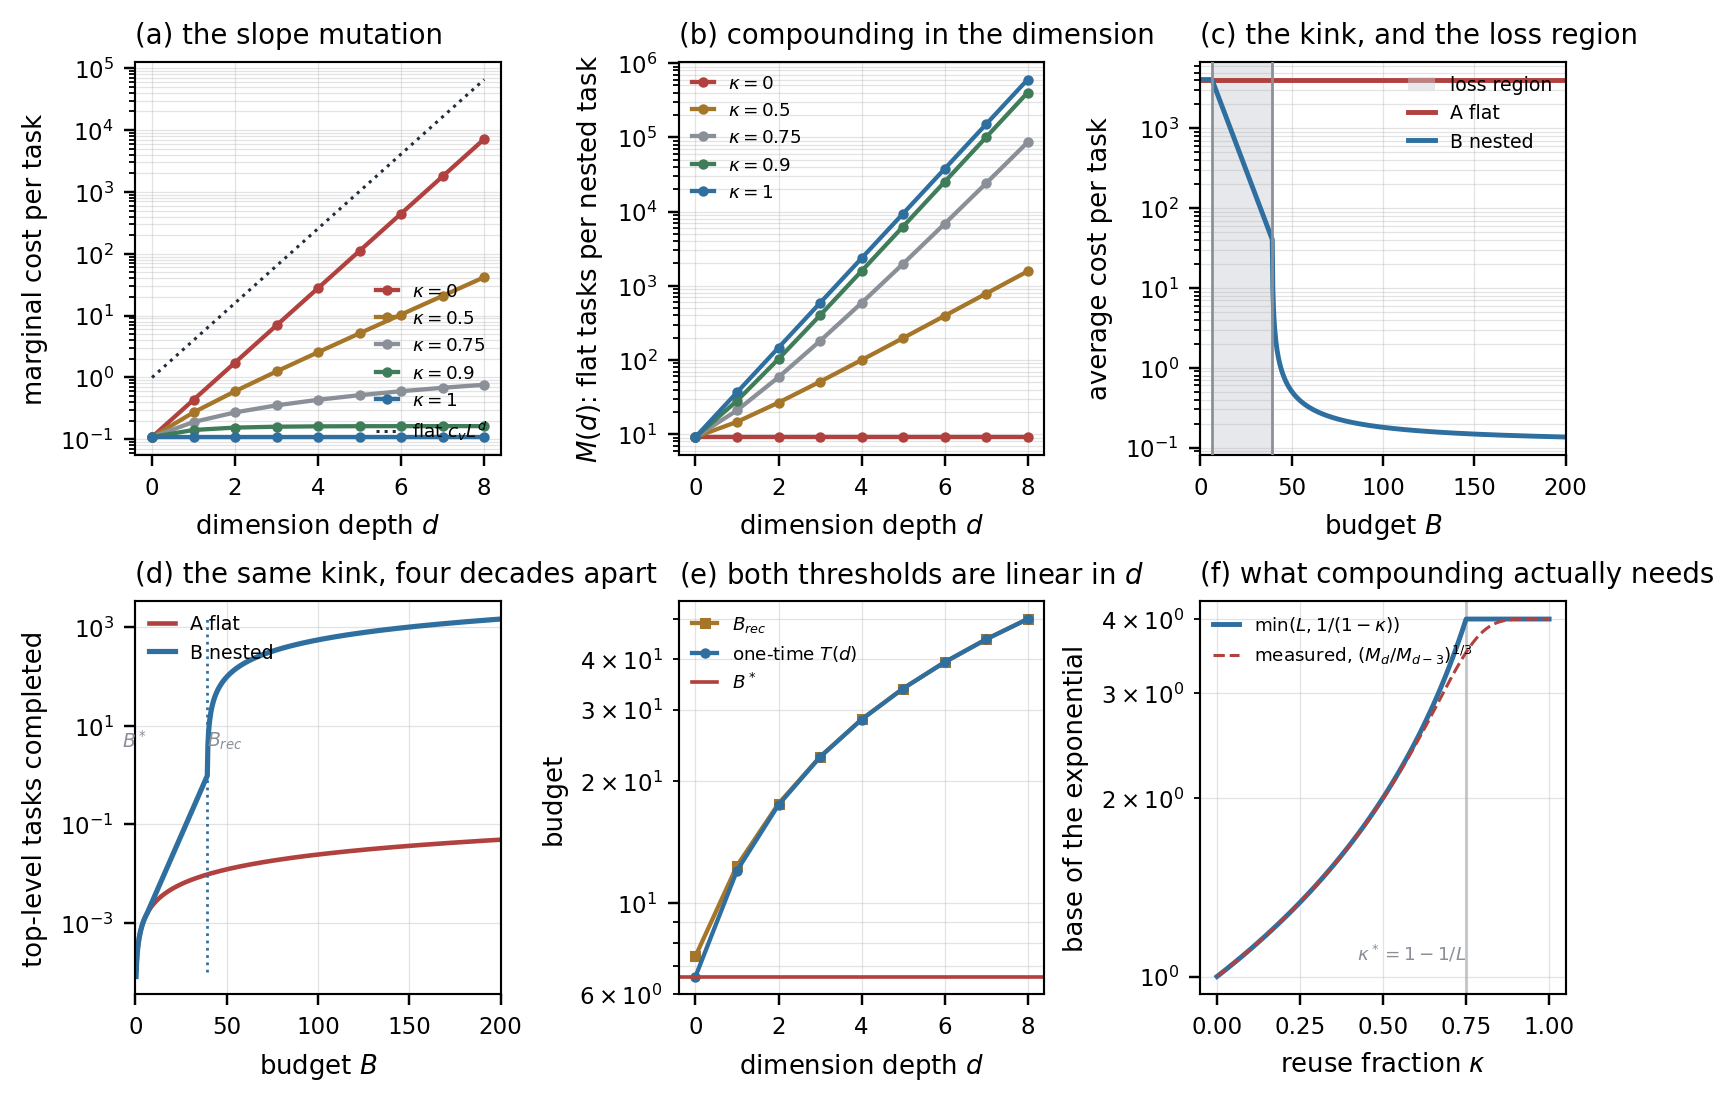
\includegraphics[width=\textwidth]{figures/nested.png}
\caption{Experiment K. (a)~Marginal cost of one task against dimension depth $d$
at five reuse rates. The flat arm is $c_vL^{d}$; $\kappa=0$ tracks it exactly up
to the constant $\bar c$, which is what amortisation alone can do. At $\kappa=1$
the line is horizontal: the price of a task stops depending on its dimension
count. (b)~The compound multiple $M(d)$. It is flat at $G_\infty$ for
$\kappa=0$ and grows with base $L$ for $\kappa\ge\kappa^{*}$. (c)~Average cost per
task against budget, with the loss region shaded: the nested arm is undefined
there by construction, since it is paying for levels it has not finished.
(d)~Completed tasks against budget on a logarithmic axis, the same kink four
decades wide. (e)~Both thresholds against depth: linear in $d$, because the
relabelling is linear even where the task is not. (f)~The compound base against
$\kappa$: $\min(L,1/(1-\kappa))$, with the knee at $\kappa^{*}=1-1/L$ marked. The
measured values are $(M_d/M_{d-3})^{1/3}$ from panel~(b), a ratio that cancels
$G_\infty$. They sit on the prediction away from the knee; \emph{at} the knee they
sit below it, by the finite-window factor $(u_{d-3}/u_d)^{1/3}$ with
$u_d=1+\kappa d$ --- a factor that closes only as $d\to\infty$, and not a fitted
offset.}
\label{fig:nested}
\end{figure*}

\paragraph{What the compounding is not} Three limits must be stated with the
result, or the section will be read as claiming more than it shows. First,
\eqref{eq:nestedmultiple} compounds in \emph{cost} at fixed prices; it says
nothing about time, and nothing about value. If the value of a top-level task
saturates in $d$ the way reach saturates in depth --- which
\eqref{eq:cbratio} already forces at the horizon --- then the multiple in value is
capped even where the multiple in cost is not, and the two must not be quoted as
one. Second, $\kappa$ is an assumption in this experiment and a measurand in the
next; the simulation checks that the tree walk prices the recursion it claims to
price, which is a consistency result, not evidence that any compiler discharges
three quarters of its children's checks. Third, the loss region is not a
technicality: a system that buys a hierarchy and never runs enough tasks to
amortise \eqref{eq:nestedbuild} is \emph{worse} than one that never built it, and
$B_{\text{rec}}$ says by how much budget. High reuse makes the upper layer eat the
lower layer's complexity; it does not make the purchase free.

\subsection{Is AI OS the next crossing?}

The model makes a specific claim about what comes after a crossing: the new gap is
inside the space just connected, it is strictly narrower, and it inherits the reach.
After biology crossed the quantum gap, the next gap is not ``more quantum
coherence''; it is \emph{how to build the structure instead of growing it}---the
biomimetic-materials problem. Evolution had a billion years and a population to
search with; a laboratory has neither, which is why the successor difficulty is
higher even though the physics is easier to describe.

The same structure applies to agent systems. For a semantic layer, the narrow
condition is roughly ``a machine can hold and re-check a claim across a context
boundary'', and the quantity that governs reach is not raw model capability but
\emph{witness density}: the fraction of claims that arrive with an artefact a third
party could check. Under \eqref{eq:k}, a system with high fidelity and a
high-density witness trail has a small exponent and therefore large reach, while a
system with better benchmarks but a sparse trail has a large exponent and stays
narrow. This remains a conjecture: \S\ref{sec:emergence} tests the weaker claim that
a scaling law can be \emph{read} as a fidelity curve, and finds the reading
consistent but unable to discriminate; it says nothing about witness density. It is
stated because it is falsifiable---measure witness density and reach
independently in deployed systems, and the model predicts they covary with the
exponent of \eqref{eq:k} rather than with capability.

\subsection{Threats to validity}
\label{sec:threats}

\begin{enumerate}
\item \textbf{The experiments validate a model, not nature.} The power law is
derived; the simulation confirms that the implementation realises it and locates
where it stops. The physical content rests on four literature anchors, and on one
assumed reach anchor which we swept.
\item \textbf{The inverse-rarity assumption is an assumption.} Equation
\eqref{eq:amp} is a modelling choice with a plausible story, not a thermodynamic
result. A different rarity model would change \eqref{eq:k}.
\item \textbf{The room-temperature coherence claim is contested.} We encode the
sceptical reading \cite{duan2017}. Adopting the optimistic reading
\cite{panitchayangkoon2010} would strengthen the biological reach result and weaken
our argument that reach is independent of coherence---so the sceptical choice is
the conservative one for our thesis.
\item \textbf{Slack noise is assumed proportional to remaining room.} An absolute
$\sigma$ would be unphysical at high fidelity; the proportionality constant is not
measured.
\item \textbf{The span horizon censors \num{25.6}\% of crossings.} Those rows are
excluded from regression rather than clipped, which biases nothing but discards a
quarter of the sample.
\item \textbf{One gap at a time.} The model has no networks, no shared conditions,
and no cost coupling between crossings. A system of interacting gaps is future work.
\item \textbf{Three of the four boundary fidelities are assumptions.} Experiment~D
rests on a table in which one number is measured. The ordering of the four
boundaries is robust to moving any assumption by a factor of two; the statement
that \emph{no} boundary is seamless is not, because the quantum boundary is
\num{0.30} nines from the threshold. We report the margin for that reason.
\item \textbf{The noise model is linear and complementary.} It assumes a boundary
passes the condition with probability $F$ and everything else with probability
$1-F$. A real filter's pass and stop bands are not exact complements, and the
cryostat/scaffold contrast is precisely where they diverge---a cryostat rejects
noise by rejecting nearly everything, including its own support infrastructure.
The \emph{ratios} in Table~\ref{tab:noise} survive that objection; the absolute
over-budget factors do not.
\item \textbf{Selectivity is not boundary fidelity.} The two are distinguished in
\S\ref{sec:fidelity} and \S\ref{sec:limit}, but the engine's single
``amplification'' field still mixes them with multiplicity. Experiment~E works in
the law's own units for that reason, and compares exponents rather than absolute
reach.
\item \textbf{Experiment~F rests on an untested bridge.} Equation~\eqref{eq:bridge}
converts a per-token loss into a boundary fidelity, and no scaling-law measurement
can validate that conversion: a systematic error in it moves every number in
\S\ref{sec:emergence} while leaving every fit statistic unchanged. What the
experiment does establish does not depend on the bridge's \emph{form}, only on
$F$ being a per-boundary probability composed multiplicatively---which is what the
depth-width prediction tests.
\item \textbf{The emergence section inherits the scaling law's own disputes.} The
two laws carried differ in exponent by \num{\emExponentRatio}; we report both
rather than choosing, but a third law would give a third $k$.
\item \textbf{A hash witnesses a state, not an action.} This is the sharpest limit
in \S\ref{sec:causal} and no implementation removes it. An agent that finds the
intended artefact already in place and does nothing produces a witness matching
the intent, and the two histories are indistinguishable because they \emph{are}
the same final state. The measured zero false-completion rate is therefore a
property of a model in which every failure changes the state; a failure that
preserves it is unobservable in principle rather than merely unobserved.
\item \textbf{The witness is only as strong as its registration.} The intended
digest has to arrive from outside the run. Poison that supply and the membrane
certifies whatever is on disk, because a hash compared against an expectation
derived from itself is the tautology it appears to be. A guarantee that holds only
for honest registration is a guarantee about the registrar, and the mechanism by
which a registrar is kept honest is not something this paper supplies.
\item \textbf{The weak baseline is a keyword scan, deliberately.} \S\ref{sec:causal}
compares the causal judge against a rule that looks for error strings, not against
a language model reading the log. A stronger reader would move
\num{\cgWeakFcr}\% but not the ceiling, which is set by what the harness emits; the
choice is made so that the causal result cannot be an artefact of a weak opponent.
It is not evidence that any particular LLM judge is as poor as the scan.
\item \textbf{One failure mechanism per task.} The generative model draws a single
failure mode, so the measured channels do not overlap and their contributions add.
A system that fails twice, once visibly and once silently, would show a lower
causal sensitivity than reported here, and by an amount this experiment does not
bound.
\end{enumerate}

\section{Conclusion}
\label{sec:concl}

An interface is not a published surface. It is a narrowing condition whose
satisfaction buys reach, and the price of the crossing is set by the mechanism
rather than by the gap. Formalising this yields a law with a testable shape:
$\mathrm{Reach}\propto(1-D)^{-k}$ with $k=\gamma P_0\lvert\ln s\rvert$, a family
indexed by fidelity rather than a single curve.

Across \num{7000} simulated crossings, the family is recovered to within
\num{0.4}\% and the single curve is rejected at $R^2=0.12$. The counterfactual is
the sharpest result: a mechanism that extends coherence by nine orders of magnitude
gains two orders of reach, while a mechanism that extends it by nothing gains five,
because replicability---not coherence---sets the scale. The failure boundary is the
mechanism's own fidelity, and the fractal ladder terminates at a representational
ceiling of $1-10^{-9}$, \num{24} generations from $D=0.99$.

Two further results are not fits but small theorems, and they explain why the
numbers above look the way they do. Seamlessness is a threshold on resistance, so
it arrives in whole nines: a boundary at $1.9$ nines is not nearly transparent but
not transparent, and a five-stratum stack cannot be made seamless by improving one
boundary, because depth costs $\log_{10}n$ extra nines. And the exponential form
of the law is a local truth---exact in the narrowing coordinate and along the
ladder, tangent in difficulty with a rate $k/(1-D)$ that diverges, and impossible
globally with a constant rate because $\ln\mathrm{Reach}$ is strictly convex.
Reach does grow explosively near $D=1$. What a single $\alpha$ describes is the
tangent, and a paper that reports one has measured the curve's slope at a point
without measuring its curvature.

The same law was then applied to a language-model scaling law, and it is the one
place where the model was turned on a claim from outside its own domain. The law
survived and the explanation did not. Reach follows the power law exactly, but the
fit discriminates nothing---$\alpha$ and $P_0$ are the only free quantities and the
law fixes their product---so the falsifiable content is the implied selectivity,
$s=0.46$. The critical scale near \num{20}B is real and reproducible, but at it the
boundary is at \num{\emNinesTwenty} nines rather than the two nines the hypothesis
requires; two nines lie \num{\emPtweFactor} times further out. What the model does
contribute is a reason for the step's \emph{appearance}: composing boundaries
translates the accuracy curve without steepening it, so every task depth shows the
same \num{\emWidth}-decade transition, and sampling model sizes a decade apart puts
four points inside it. That is a claim with a number, and it fails if a deeper task
shows a narrower transition.

The last experiment turns the same instrument on the paper's own remedy. A
witnessed system does not convert depth into an explosion, and cannot: completion
of a ladder is bounded by completion of its prefixes, so reach is non-increasing in
depth whatever the per-layer law is. What the label buys is not reach but the
absence of an invented one---at $D=0.99$ and depth \teDepthMax{} the transcript
overstates the causal rate by \teInflationDeep, while the label's genuine gain is
\teBOrders{} orders of magnitude in the \emph{cost of depth}. A discount belongs at
the margin, where it can be spent; spent on the exponent it would be a different
claim, and one the arithmetic does not permit.

That discount, priced, splits in two. On a single interface it is arithmetic: a
compiled traverse costs $\bar c$ instead of $c_v$, and no budget turns a price ratio
into an exponent. Across layers it is not arithmetic, because a compiled layer can
be \emph{cited} by the layer above it, and citation is what removes the dimension
count from the price. Writing $\kappa$ for the reuse rate---the fraction of a
child's verification its parent's label discharges---the marginal cost of a task at
depth $d$ obeys $m_d=\kappa\bar c+(1-\kappa)Lm_{d-1}$, so the advantage over
independent verification grows with base $\min(L,1/(1-\kappa))$: exactly $G_\infty$
at $\kappa=0$, and $L$ for any $\kappa\ge\kappa^{*}=1-1/L$. A system below the knee
compounds nothing however much it compiles, and a system above it gains nothing
further by compiling harder. Economically this is the content of seamlessness:
high reuse lets the upper layer's marginal cost swallow the lower layer's
complexity, which is why a transparent interface is worth building and a merely
fast one is not. The budget that buys that position is not $B^{*}$ alone; the
relabelling is paid per level, so the arm is strictly behind between $B^{*}$ and
$B_{\text{rec}}(d)=T(d)/[1-m_d/c_{\text{flat}}(d)]$, and a hierarchy bought and
never exercised is worse than none.

The honest summary is narrower than the ambition. What has been shown is that a
particular formalisation of interfaces is internally consistent, that its central
law is recovered numerically to within a fraction of a percent, that its exponent
is mechanism-specific, and that it breaks in two places that can be located
exactly. What has not been shown is that the physical anchors are right, or that
inverse rarity is the correct model of reach. Both are stated as assumptions above,
and both are the experiments we would run next.

% A fresh page, so the appendix cannot begin under a float that belongs
% to the conclusion's page and be read before its own heading.
\clearpage
\appendices
\section{Self-Audit of this Paper}
\label{app:selfaudit}

A package built to refuse unwitnessed claims should not publish a manuscript that
never turns that refusal on itself. So the audit was run on the paper. The
instrument is \texttt{experiments/paper\_self\_audit.py}: it reads this file,
locates each claim by a pattern that must match exactly once, re-derives the
numbers printed above from the modules that generated them, and writes the table
and counts below. If an anchor moves, or a module and its macro disagree, the audit
fails instead of quietly reporting on a paper it did not read. It reports
\saClaimCount{} claims: \saPassCount{} \textsc{pass}, \saInvalidCount{}
\textsc{invalid}, \saUnavailableCount{} \textsc{unavailable}, \saBlindCount{}
\textsc{blind}, and \saFailCount{} escalated to failure.

\paragraph{What each verdict is allowed to mean} The four values are the package's
own, and their scope is quoted rather than paraphrased. \textsc{pass} in
Table~\ref{tab:selfaudit} is mechanical: the printed number and the module that
produced it agree at the printed precision, and for the knee the check re-tests the
property as well as the value, because a number that bounds nothing would still
print $0.75$. It does not mean the model is right about the world; it means a
reader who checks the arithmetic will find it holding. \textsc{invalid} means no
witness was offered---\emph{nothing to examine}, which is a different finding from
\emph{refuted} and is kept apart from it here for the same reason the engine keeps
it apart everywhere else. \textsc{unavailable} means the instrument that could
answer does not exist in this setting, and an environment that cannot answer must
not be allowed to accuse. \textsc{blind} is a statement about the registry's
coverage, not about nature.

\begin{table}[h!]
\centering
\caption{Self-audit of this paper. Each claim was graded with the same lattice the
paper applies to other people's filings, against the evidence channel in the last
column. A \textsc{pass} means the manuscript's arithmetic recomputes, not that the
claim is true of nature; an \textsc{invalid} means no witness was offered, not that
the claim is false.}
\label{tab:selfaudit}
\footnotesize
% generated by experiments/paper_self_audit.py -- do not edit
\setlength{\tabcolsep}{4pt}
\begin{tabular}{@{}>{\raggedright\arraybackslash}p{0.05\columnwidth}>{\raggedright\arraybackslash}p{0.28\columnwidth}>{\raggedright\arraybackslash}p{0.22\columnwidth}>{\raggedright\arraybackslash}p{0.30\columnwidth}@{}}
\toprule
id & claim & verdict & evidence channel \\
\midrule
A1 & The critical-budget closed form & \textsc{pass} & recomputation from experiments/\allowbreak{}critical\_\allowbreak{}budget\_\allowbreak{}experiment.py \\
A2 & The amortisation ceiling & \textsc{pass} & recomputation, printed by two independent generators \\
A3 & The slope nothing was fitted to & \textsc{pass} & recomputation from the two prices \\
A4 & The reuse knee, with bounded marginal cost above it & \textsc{pass} & recomputation plus a two-sided boundedness test \\
A5 & The recovery budget & \textsc{pass} & recomputation, plus the inequality B\_\allowbreak{}rec \textgreater{} T \\
A6 & The efficiency jump at B=200 & \textsc{pass} & recomputation, and a read-back of the generated table \\
A7 & The reach advantage peaks inside and returns to one & \textsc{pass} & numerical re-solution, no generated constant involved \\
B1 & Causation is labelling: the do-operator separates the two probabilities & \textsc{unavailable} & no instrument: the do-operator is estimated inside a simulated judge, not in a physical system \\
B2 & An interface is a boundary, not a surface & \textsc{unavailable} & definitional: no measurement could decide it \\
C1 & The per-layer success probability is 1 minus the difficulty & \textsc{invalid} & no witness: no measurement of a per-layer success rate at any of the five scales \\
C2 & Reach tracks witness density, not capability & \textsc{invalid} & no witness: stated as a conjecture, no deployed system measured \\
D1 & Scale partitions into the five strata & \textsc{blind} & registry statement: coverage of the strata graph, not of nature \\
\bottomrule
\end{tabular}

\end{table}

\paragraph{The two premises we cannot test} The reading of an interface as a
boundary, and of causation as labelling, are the axioms the model is built on. No
experiment inside this paper could decide either, and a paper that claimed to have
decided one would be the exact artefact the rest of this work refuses. Both are
recorded as \textsc{unavailable}: \emph{This is a philosophical premise, not a
falsifiable hypothesis.} They are printed here rather than buried because a reader
is entitled to know which of the paper's load-bearing statements are definitions,
and because a premise that is invisible is one that gets cited as a result.

\paragraph{The two assumptions we have not measured} The per-layer success
probability is set to $p_{\text{layer}}=1-D$. That is a choice, it is stated as one
in Section~\ref{sec:emergence}, and every ordering reported there survives any
monotone decreasing replacement; but no measurement of a per-layer success rate
exists at any of the five scales, so the row is \textsc{invalid}---unwitnessed, not
wrong. The conjecture that reach tracks witness density rather than capability is
likewise \textsc{invalid}: it is falsifiable and has not been falsified, which is a
different and better position than the two premises above, and the difference is
the reason the values are kept distinct.

\paragraph{The partition we cannot see past} Scale is partitioned into
\saStrataCount{} strata joined by \saEdgeCount{} boundaries. Of the
\saPairCount{} unordered pairs this admits, \saUnwitnessedCount{} have no filing
and therefore no witness, and whether a sixth stratum exists is a question the
registry cannot pose at all. That is a gap in the taxonomy, not evidence that the
missing boundaries are uncrossable, and it is why the row is \textsc{blind} rather
than a failure.

\paragraph{What the exercise cost} One audit implementation bug, found by the audit
itself: the first version tested the knee's claim by checking that the marginal
cost was ``large'' below $\kappa^{*}$, which failed on a true statement because
growth is geometric, not explosive. The test now checks the recursion identity
$({m_d-\kappa\bar c})/{m_{d-1}}=(1-\kappa)L$ exactly. The episode is reported
because an auditor whose own errors are invisible has no standing to report anyone
else's, and because the corrected check is the one printed above.

\subsection{Auditing the Bibliography}
\label{sec:bibaudit}

The claims above are the paper's arguments. Its citations are claims of a different
kind---\emph{this identifier names this paper}---and they are the ones an author is
most able to get wrong by accident and most tempted to leave unchecked. We ran our
own \texttt{CitationAuditProxy} against the \texttt{references.bib} of this paper:
each entry's DOI is resolved against CrossRef and each arXiv id against the arXiv
API, and the record's returned title is compared with the title the entry claims.
That comparison is the witness. Nothing about the manuscript is consulted.

Of the \caTotal{} entries, \caPass{} are \textsc{pass}: an agency answered and the
title matched (\caCrossrefCount{} through CrossRef, \caArxivCount{} through arXiv),
and \caInvalid{} could not be witnessed at all. The \textsc{fail} count is
\caFail{}, the verdict that would matter most: a right-looking identifier that
resolves to a different paper is the fabrication this audit exists to catch, and
none was found---a statement about this bibliography and not about bibliographies
in general. Both \textsc{invalid} entries are genuinely unwitnessable: a 1982 book,
and a 1962 print article from a journal volume that predates DOI registration. No
agency can ever speak for either, so deleting them to make the table green would be
the same false completion the rest of this work refuses. They are kept, and their
existence is recorded as a \emph{locator}---a catalogue record for the book, a
scanned volume index for the article---so that the reader can go and look rather
than take our word. A locator is not a witness, and Table~\ref{tab:bibaudit} keeps
the two apart.

\paragraph{The first run was the finding} On its first run the auditor returned
\caPriorPass{} \textsc{pass} and \caPriorInvalid{} \textsc{invalid}, with no
\textsc{fail}. Not one entry carried a DOI or an arXiv id: the bibliography was a
set of assertions that nothing outside itself could check, which is precisely the
shape of claim this package exists to distrust. The verdict was not that the
citations were false but that they were unwitnessable, and the repair was to give
each one the identifier under which it could be re-resolved. The zero \textsc{fail}
in that run is not praise: with no identifier present there was nothing to
contradict. The pre-audit file is kept as
\texttt{data/references\_pre\_audit.bib} so that the claim can be re-run rather
than believed.

\paragraph{How the identifiers were chosen} By title search, not by memory, and
the distinction earned its keep: for most entries the first hit returned by the
agency was a \emph{different} paper with a similar title---a different spectroscopy
review, a different complexity essay, a 2024 paper about proteins rather than
language models. Each candidate was accepted only after the auditor's own title
comparison passed. A search that returns a plausible DOI is not a witness; a record
whose title is the entry's title is.

\begin{table}[h!]
\centering
\caption{Bibliography audit. The verdict column is the auditor's own; the last
column distinguishes an entry an agency witnessed from one a human located. A
\textsc{pass} means the identifier resolved and the returned title matched, not
that the paper is correct.}
\label{tab:bibaudit}
\footnotesize
% generated by experiments/citation_audit_report.py -- do not edit
\setlength{\tabcolsep}{3pt}
\scriptsize
\begin{tabular}{@{}>{\raggedright\arraybackslash}p{0.24\columnwidth}>{\raggedright\arraybackslash}p{0.24\columnwidth}>{\raggedright\arraybackslash}p{0.16\columnwidth}>{\raggedright\arraybackslash}p{0.26\columnwidth}@{}}
\toprule
entry & identifier & verdict & how it was witnessed \\
\midrule
engel\allowbreak{}2007 & 10.\allowbreak{}1038/\allowbreak{}nature\allowbreak{}05678 & \textsc{pass} & crossref (title match) \\
brixner\allowbreak{}2005 & 10.\allowbreak{}1038/\allowbreak{}nature\allowbreak{}03429 & \textsc{pass} & crossref (title match) \\
panitchayangkoon\allowbreak{}2010 & 10.\allowbreak{}1073/\allowbreak{}pnas.\allowbreak{}1005484107 & \textsc{pass} & crossref (title match) \\
duan\allowbreak{}2017 & 10.\allowbreak{}1073/\allowbreak{}pnas.\allowbreak{}1702261114 & \textsc{pass} & crossref (title match) \\
adolphs\allowbreak{}2006 & 10.\allowbreak{}1529/\allowbreak{}biophysj.\allowbreak{}105.\allowbreak{}079483 & \textsc{pass} & crossref (title match) \\
mohseni\allowbreak{}2008 & 10.\allowbreak{}1063/\allowbreak{}1.\allowbreak{}3002335 & \textsc{pass} & crossref (title match) \\
plenio\allowbreak{}2008 & 10.\allowbreak{}1088/\allowbreak{}1367-\allowbreak{}2630/\allowbreak{}10/\allowbreak{}11/\allowbreak{}113019 & \textsc{pass} & crossref (title match) \\
lambert\allowbreak{}2013 & 10.\allowbreak{}1038/\allowbreak{}nphys\allowbreak{}2474 & \textsc{pass} & crossref (title match) \\
romero\allowbreak{}2017 & 10.\allowbreak{}1038/\allowbreak{}nature\allowbreak{}22012 & \textsc{pass} & crossref (title match) \\
kjaergaard\allowbreak{}2020 & 10.\allowbreak{}1146/\allowbreak{}annurev-\allowbreak{}conmatphys-\allowbreak{}031119-\allowbreak{}050605 & \textsc{pass} & crossref (title match) \\
mandelbrot\allowbreak{}1982 & -- & \textsc{invalid} & no agency; located at OpenLibrary work OL1808391W \\
simon\allowbreak{}1962 & -- & \textsc{invalid} & no agency; located at archive.org scan of Proc. Am. Phil. Soc. Vol. 106 (1962), index p. 467 \\
west\allowbreak{}1997 & 10.\allowbreak{}1126/\allowbreak{}science.\allowbreak{}276.\allowbreak{}5309.\allowbreak{}122 & \textsc{pass} & crossref (title match) \\
barabasi\allowbreak{}1999 & 10.\allowbreak{}1126/\allowbreak{}science.\allowbreak{}286.\allowbreak{}5439.\allowbreak{}509 & \textsc{pass} & crossref (title match) \\
clauset\allowbreak{}2009 & 10.\allowbreak{}1137/\allowbreak{}070710111 & \textsc{pass} & crossref (title match) \\
hoffmann\allowbreak{}2022 & 2203.\allowbreak{}15556 & \textsc{pass} & arxiv (title match) \\
kaplan\allowbreak{}2020 & 2001.\allowbreak{}08361 & \textsc{pass} & arxiv (title match) \\
schaeffer\allowbreak{}2023 & 2304.\allowbreak{}15004 & \textsc{pass} & arxiv (title match) \\
besiroglu\allowbreak{}2024 & 2404.\allowbreak{}10102 & \textsc{pass} & arxiv (title match) \\
\bottomrule
\end{tabular}

\end{table}

\bibliographystyle{IEEEtran}
\bibliography{references}

\end{document}
